\documentclass{article} % For LaTeX2e
\usepackage{iclr2019_conference,times}
\usepackage{graphicx} % more modern
\usepackage{subfigure}
\usepackage{hhline}

% Optional math commands from https://github.com/goodfeli/dlbook_notation.
%%%%% NEW MATH DEFINITIONS %%%%%

\usepackage{amsmath,amsfonts,bm}

% Mark sections of captions for referring to divisions of figures
\newcommand{\figleft}{{\em (Left)}}
\newcommand{\figcenter}{{\em (Center)}}
\newcommand{\figright}{{\em (Right)}}
\newcommand{\figtop}{{\em (Top)}}
\newcommand{\figbottom}{{\em (Bottom)}}
\newcommand{\captiona}{{\em (a)}}
\newcommand{\captionb}{{\em (b)}}
\newcommand{\captionc}{{\em (c)}}
\newcommand{\captiond}{{\em (d)}}

% Highlight a newly defined term
\newcommand{\newterm}[1]{{\bf #1}}


% Figure reference, lower-case.
\def\figref#1{figure~\ref{#1}}
% Figure reference, capital. For start of sentence
\def\Figref#1{Figure~\ref{#1}}
\def\twofigref#1#2{figures \ref{#1} and \ref{#2}}
\def\quadfigref#1#2#3#4{figures \ref{#1}, \ref{#2}, \ref{#3} and \ref{#4}}
% Section reference, lower-case.
\def\secref#1{section~\ref{#1}}
% Section reference, capital.
\def\Secref#1{Section~\ref{#1}}
% Reference to two sections.
\def\twosecrefs#1#2{sections \ref{#1} and \ref{#2}}
% Reference to three sections.
\def\secrefs#1#2#3{sections \ref{#1}, \ref{#2} and \ref{#3}}
% Reference to an equation, lower-case.
\def\eqref#1{equation~\ref{#1}}
% Reference to an equation, upper case
\def\Eqref#1{Equation~\ref{#1}}
% A raw reference to an equation---avoid using if possible
\def\plaineqref#1{\ref{#1}}
% Reference to a chapter, lower-case.
\def\chapref#1{chapter~\ref{#1}}
% Reference to an equation, upper case.
\def\Chapref#1{Chapter~\ref{#1}}
% Reference to a range of chapters
\def\rangechapref#1#2{chapters\ref{#1}--\ref{#2}}
% Reference to an algorithm, lower-case.
\def\algref#1{algorithm~\ref{#1}}
% Reference to an algorithm, upper case.
\def\Algref#1{Algorithm~\ref{#1}}
\def\twoalgref#1#2{algorithms \ref{#1} and \ref{#2}}
\def\Twoalgref#1#2{Algorithms \ref{#1} and \ref{#2}}
% Reference to a part, lower case
\def\partref#1{part~\ref{#1}}
% Reference to a part, upper case
\def\Partref#1{Part~\ref{#1}}
\def\twopartref#1#2{parts \ref{#1} and \ref{#2}}

\def\ceil#1{\lceil #1 \rceil}
\def\floor#1{\lfloor #1 \rfloor}
\def\1{\bm{1}}
\newcommand{\train}{\mathcal{D}}
\newcommand{\valid}{\mathcal{D_{\mathrm{valid}}}}
\newcommand{\test}{\mathcal{D_{\mathrm{test}}}}

\def\eps{{\epsilon}}


% Random variables
\def\reta{{\textnormal{$\eta$}}}
\def\ra{{\textnormal{a}}}
\def\rb{{\textnormal{b}}}
\def\rc{{\textnormal{c}}}
\def\rd{{\textnormal{d}}}
\def\re{{\textnormal{e}}}
\def\rf{{\textnormal{f}}}
\def\rg{{\textnormal{g}}}
\def\rh{{\textnormal{h}}}
\def\ri{{\textnormal{i}}}
\def\rj{{\textnormal{j}}}
\def\rk{{\textnormal{k}}}
\def\rl{{\textnormal{l}}}
% rm is already a command, just don't name any random variables m
\def\rn{{\textnormal{n}}}
\def\ro{{\textnormal{o}}}
\def\rp{{\textnormal{p}}}
\def\rq{{\textnormal{q}}}
\def\rr{{\textnormal{r}}}
\def\rs{{\textnormal{s}}}
\def\rt{{\textnormal{t}}}
\def\ru{{\textnormal{u}}}
\def\rv{{\textnormal{v}}}
\def\rw{{\textnormal{w}}}
\def\rx{{\textnormal{x}}}
\def\ry{{\textnormal{y}}}
\def\rz{{\textnormal{z}}}

% Random vectors
\def\rvepsilon{{\mathbf{\epsilon}}}
\def\rvtheta{{\mathbf{\theta}}}
\def\rva{{\mathbf{a}}}
\def\rvb{{\mathbf{b}}}
\def\rvc{{\mathbf{c}}}
\def\rvd{{\mathbf{d}}}
\def\rve{{\mathbf{e}}}
\def\rvf{{\mathbf{f}}}
\def\rvg{{\mathbf{g}}}
\def\rvh{{\mathbf{h}}}
\def\rvu{{\mathbf{i}}}
\def\rvj{{\mathbf{j}}}
\def\rvk{{\mathbf{k}}}
\def\rvl{{\mathbf{l}}}
\def\rvm{{\mathbf{m}}}
\def\rvn{{\mathbf{n}}}
\def\rvo{{\mathbf{o}}}
\def\rvp{{\mathbf{p}}}
\def\rvq{{\mathbf{q}}}
\def\rvr{{\mathbf{r}}}
\def\rvs{{\mathbf{s}}}
\def\rvt{{\mathbf{t}}}
\def\rvu{{\mathbf{u}}}
\def\rvv{{\mathbf{v}}}
\def\rvw{{\mathbf{w}}}
\def\rvx{{\mathbf{x}}}
\def\rvy{{\mathbf{y}}}
\def\rvz{{\mathbf{z}}}

% Elements of random vectors
\def\erva{{\textnormal{a}}}
\def\ervb{{\textnormal{b}}}
\def\ervc{{\textnormal{c}}}
\def\ervd{{\textnormal{d}}}
\def\erve{{\textnormal{e}}}
\def\ervf{{\textnormal{f}}}
\def\ervg{{\textnormal{g}}}
\def\ervh{{\textnormal{h}}}
\def\ervi{{\textnormal{i}}}
\def\ervj{{\textnormal{j}}}
\def\ervk{{\textnormal{k}}}
\def\ervl{{\textnormal{l}}}
\def\ervm{{\textnormal{m}}}
\def\ervn{{\textnormal{n}}}
\def\ervo{{\textnormal{o}}}
\def\ervp{{\textnormal{p}}}
\def\ervq{{\textnormal{q}}}
\def\ervr{{\textnormal{r}}}
\def\ervs{{\textnormal{s}}}
\def\ervt{{\textnormal{t}}}
\def\ervu{{\textnormal{u}}}
\def\ervv{{\textnormal{v}}}
\def\ervw{{\textnormal{w}}}
\def\ervx{{\textnormal{x}}}
\def\ervy{{\textnormal{y}}}
\def\ervz{{\textnormal{z}}}

% Random matrices
\def\rmA{{\mathbf{A}}}
\def\rmB{{\mathbf{B}}}
\def\rmC{{\mathbf{C}}}
\def\rmD{{\mathbf{D}}}
\def\rmE{{\mathbf{E}}}
\def\rmF{{\mathbf{F}}}
\def\rmG{{\mathbf{G}}}
\def\rmH{{\mathbf{H}}}
\def\rmI{{\mathbf{I}}}
\def\rmJ{{\mathbf{J}}}
\def\rmK{{\mathbf{K}}}
\def\rmL{{\mathbf{L}}}
\def\rmM{{\mathbf{M}}}
\def\rmN{{\mathbf{N}}}
\def\rmO{{\mathbf{O}}}
\def\rmP{{\mathbf{P}}}
\def\rmQ{{\mathbf{Q}}}
\def\rmR{{\mathbf{R}}}
\def\rmS{{\mathbf{S}}}
\def\rmT{{\mathbf{T}}}
\def\rmU{{\mathbf{U}}}
\def\rmV{{\mathbf{V}}}
\def\rmW{{\mathbf{W}}}
\def\rmX{{\mathbf{X}}}
\def\rmY{{\mathbf{Y}}}
\def\rmZ{{\mathbf{Z}}}

% Elements of random matrices
\def\ermA{{\textnormal{A}}}
\def\ermB{{\textnormal{B}}}
\def\ermC{{\textnormal{C}}}
\def\ermD{{\textnormal{D}}}
\def\ermE{{\textnormal{E}}}
\def\ermF{{\textnormal{F}}}
\def\ermG{{\textnormal{G}}}
\def\ermH{{\textnormal{H}}}
\def\ermI{{\textnormal{I}}}
\def\ermJ{{\textnormal{J}}}
\def\ermK{{\textnormal{K}}}
\def\ermL{{\textnormal{L}}}
\def\ermM{{\textnormal{M}}}
\def\ermN{{\textnormal{N}}}
\def\ermO{{\textnormal{O}}}
\def\ermP{{\textnormal{P}}}
\def\ermQ{{\textnormal{Q}}}
\def\ermR{{\textnormal{R}}}
\def\ermS{{\textnormal{S}}}
\def\ermT{{\textnormal{T}}}
\def\ermU{{\textnormal{U}}}
\def\ermV{{\textnormal{V}}}
\def\ermW{{\textnormal{W}}}
\def\ermX{{\textnormal{X}}}
\def\ermY{{\textnormal{Y}}}
\def\ermZ{{\textnormal{Z}}}

% Vectors
\def\vzero{{\bm{0}}}
\def\vone{{\bm{1}}}
\def\vmu{{\bm{\mu}}}
\def\vtheta{{\bm{\theta}}}
\def\va{{\bm{a}}}
\def\vb{{\bm{b}}}
\def\vc{{\bm{c}}}
\def\vd{{\bm{d}}}
\def\ve{{\bm{e}}}
\def\vf{{\bm{f}}}
\def\vg{{\bm{g}}}
\def\vh{{\bm{h}}}
\def\vi{{\bm{i}}}
\def\vj{{\bm{j}}}
\def\vk{{\bm{k}}}
\def\vl{{\bm{l}}}
\def\vm{{\bm{m}}}
\def\vn{{\bm{n}}}
\def\vo{{\bm{o}}}
\def\vp{{\bm{p}}}
\def\vq{{\bm{q}}}
\def\vr{{\bm{r}}}
\def\vs{{\bm{s}}}
\def\vt{{\bm{t}}}
\def\vu{{\bm{u}}}
\def\vv{{\bm{v}}}
\def\vw{{\bm{w}}}
\def\vx{{\bm{x}}}
\def\vy{{\bm{y}}}
\def\vz{{\bm{z}}}

% Elements of vectors
\def\evalpha{{\alpha}}
\def\evbeta{{\beta}}
\def\evepsilon{{\epsilon}}
\def\evlambda{{\lambda}}
\def\evomega{{\omega}}
\def\evmu{{\mu}}
\def\evpsi{{\psi}}
\def\evsigma{{\sigma}}
\def\evtheta{{\theta}}
\def\eva{{a}}
\def\evb{{b}}
\def\evc{{c}}
\def\evd{{d}}
\def\eve{{e}}
\def\evf{{f}}
\def\evg{{g}}
\def\evh{{h}}
\def\evi{{i}}
\def\evj{{j}}
\def\evk{{k}}
\def\evl{{l}}
\def\evm{{m}}
\def\evn{{n}}
\def\evo{{o}}
\def\evp{{p}}
\def\evq{{q}}
\def\evr{{r}}
\def\evs{{s}}
\def\evt{{t}}
\def\evu{{u}}
\def\evv{{v}}
\def\evw{{w}}
\def\evx{{x}}
\def\evy{{y}}
\def\evz{{z}}

% Matrix
\def\mA{{\bm{A}}}
\def\mB{{\bm{B}}}
\def\mC{{\bm{C}}}
\def\mD{{\bm{D}}}
\def\mE{{\bm{E}}}
\def\mF{{\bm{F}}}
\def\mG{{\bm{G}}}
\def\mH{{\bm{H}}}
\def\mI{{\bm{I}}}
\def\mJ{{\bm{J}}}
\def\mK{{\bm{K}}}
\def\mL{{\bm{L}}}
\def\mM{{\bm{M}}}
\def\mN{{\bm{N}}}
\def\mO{{\bm{O}}}
\def\mP{{\bm{P}}}
\def\mQ{{\bm{Q}}}
\def\mR{{\bm{R}}}
\def\mS{{\bm{S}}}
\def\mT{{\bm{T}}}
\def\mU{{\bm{U}}}
\def\mV{{\bm{V}}}
\def\mW{{\bm{W}}}
\def\mX{{\bm{X}}}
\def\mY{{\bm{Y}}}
\def\mZ{{\bm{Z}}}
\def\mBeta{{\bm{\beta}}}
\def\mPhi{{\bm{\Phi}}}
\def\mLambda{{\bm{\Lambda}}}
\def\mSigma{{\bm{\Sigma}}}

% Tensor
\DeclareMathAlphabet{\mathsfit}{\encodingdefault}{\sfdefault}{m}{sl}
\SetMathAlphabet{\mathsfit}{bold}{\encodingdefault}{\sfdefault}{bx}{n}
\newcommand{\tens}[1]{\bm{\mathsfit{#1}}}
\def\tA{{\tens{A}}}
\def\tB{{\tens{B}}}
\def\tC{{\tens{C}}}
\def\tD{{\tens{D}}}
\def\tE{{\tens{E}}}
\def\tF{{\tens{F}}}
\def\tG{{\tens{G}}}
\def\tH{{\tens{H}}}
\def\tI{{\tens{I}}}
\def\tJ{{\tens{J}}}
\def\tK{{\tens{K}}}
\def\tL{{\tens{L}}}
\def\tM{{\tens{M}}}
\def\tN{{\tens{N}}}
\def\tO{{\tens{O}}}
\def\tP{{\tens{P}}}
\def\tQ{{\tens{Q}}}
\def\tR{{\tens{R}}}
\def\tS{{\tens{S}}}
\def\tT{{\tens{T}}}
\def\tU{{\tens{U}}}
\def\tV{{\tens{V}}}
\def\tW{{\tens{W}}}
\def\tX{{\tens{X}}}
\def\tY{{\tens{Y}}}
\def\tZ{{\tens{Z}}}


% Graph
\def\gA{{\mathcal{A}}}
\def\gB{{\mathcal{B}}}
\def\gC{{\mathcal{C}}}
\def\gD{{\mathcal{D}}}
\def\gE{{\mathcal{E}}}
\def\gF{{\mathcal{F}}}
\def\gG{{\mathcal{G}}}
\def\gH{{\mathcal{H}}}
\def\gI{{\mathcal{I}}}
\def\gJ{{\mathcal{J}}}
\def\gK{{\mathcal{K}}}
\def\gL{{\mathcal{L}}}
\def\gM{{\mathcal{M}}}
\def\gN{{\mathcal{N}}}
\def\gO{{\mathcal{O}}}
\def\gP{{\mathcal{P}}}
\def\gQ{{\mathcal{Q}}}
\def\gR{{\mathcal{R}}}
\def\gS{{\mathcal{S}}}
\def\gT{{\mathcal{T}}}
\def\gU{{\mathcal{U}}}
\def\gV{{\mathcal{V}}}
\def\gW{{\mathcal{W}}}
\def\gX{{\mathcal{X}}}
\def\gY{{\mathcal{Y}}}
\def\gZ{{\mathcal{Z}}}

% Sets
\def\sA{{\mathbb{A}}}
\def\sB{{\mathbb{B}}}
\def\sC{{\mathbb{C}}}
\def\sD{{\mathbb{D}}}
% Don't use a set called E, because this would be the same as our symbol
% for expectation.
\def\sF{{\mathbb{F}}}
\def\sG{{\mathbb{G}}}
\def\sH{{\mathbb{H}}}
\def\sI{{\mathbb{I}}}
\def\sJ{{\mathbb{J}}}
\def\sK{{\mathbb{K}}}
\def\sL{{\mathbb{L}}}
\def\sM{{\mathbb{M}}}
\def\sN{{\mathbb{N}}}
\def\sO{{\mathbb{O}}}
\def\sP{{\mathbb{P}}}
\def\sQ{{\mathbb{Q}}}
\def\sR{{\mathbb{R}}}
\def\sS{{\mathbb{S}}}
\def\sT{{\mathbb{T}}}
\def\sU{{\mathbb{U}}}
\def\sV{{\mathbb{V}}}
\def\sW{{\mathbb{W}}}
\def\sX{{\mathbb{X}}}
\def\sY{{\mathbb{Y}}}
\def\sZ{{\mathbb{Z}}}

% Entries of a matrix
\def\emLambda{{\Lambda}}
\def\emA{{A}}
\def\emB{{B}}
\def\emC{{C}}
\def\emD{{D}}
\def\emE{{E}}
\def\emF{{F}}
\def\emG{{G}}
\def\emH{{H}}
\def\emI{{I}}
\def\emJ{{J}}
\def\emK{{K}}
\def\emL{{L}}
\def\emM{{M}}
\def\emN{{N}}
\def\emO{{O}}
\def\emP{{P}}
\def\emQ{{Q}}
\def\emR{{R}}
\def\emS{{S}}
\def\emT{{T}}
\def\emU{{U}}
\def\emV{{V}}
\def\emW{{W}}
\def\emX{{X}}
\def\emY{{Y}}
\def\emZ{{Z}}
\def\emSigma{{\Sigma}}

% entries of a tensor
% Same font as tensor, without \bm wrapper
\newcommand{\etens}[1]{\mathsfit{#1}}
\def\etLambda{{\etens{\Lambda}}}
\def\etA{{\etens{A}}}
\def\etB{{\etens{B}}}
\def\etC{{\etens{C}}}
\def\etD{{\etens{D}}}
\def\etE{{\etens{E}}}
\def\etF{{\etens{F}}}
\def\etG{{\etens{G}}}
\def\etH{{\etens{H}}}
\def\etI{{\etens{I}}}
\def\etJ{{\etens{J}}}
\def\etK{{\etens{K}}}
\def\etL{{\etens{L}}}
\def\etM{{\etens{M}}}
\def\etN{{\etens{N}}}
\def\etO{{\etens{O}}}
\def\etP{{\etens{P}}}
\def\etQ{{\etens{Q}}}
\def\etR{{\etens{R}}}
\def\etS{{\etens{S}}}
\def\etT{{\etens{T}}}
\def\etU{{\etens{U}}}
\def\etV{{\etens{V}}}
\def\etW{{\etens{W}}}
\def\etX{{\etens{X}}}
\def\etY{{\etens{Y}}}
\def\etZ{{\etens{Z}}}

% The true underlying data generating distribution
\newcommand{\pdata}{p_{\rm{data}}}
% The empirical distribution defined by the training set
\newcommand{\ptrain}{\hat{p}_{\rm{data}}}
\newcommand{\Ptrain}{\hat{P}_{\rm{data}}}
% The model distribution
\newcommand{\pmodel}{p_{\rm{model}}}
\newcommand{\Pmodel}{P_{\rm{model}}}
\newcommand{\ptildemodel}{\tilde{p}_{\rm{model}}}
% Stochastic autoencoder distributions
\newcommand{\pencode}{p_{\rm{encoder}}}
\newcommand{\pdecode}{p_{\rm{decoder}}}
\newcommand{\precons}{p_{\rm{reconstruct}}}

\newcommand{\laplace}{\mathrm{Laplace}} % Laplace distribution

\newcommand{\E}{\mathbb{E}}
\newcommand{\Ls}{\mathcal{L}}
\newcommand{\R}{\mathbb{R}}
\newcommand{\emp}{\tilde{p}}
\newcommand{\lr}{\alpha}
\newcommand{\reg}{\lambda}
\newcommand{\rect}{\mathrm{rectifier}}
\newcommand{\softmax}{\mathrm{softmax}}
\newcommand{\sigmoid}{\sigma}
\newcommand{\softplus}{\zeta}
\newcommand{\KL}{D_{\mathrm{KL}}}
\newcommand{\Var}{\mathrm{Var}}
\newcommand{\standarderror}{\mathrm{SE}}
\newcommand{\Cov}{\mathrm{Cov}}
% Wolfram Mathworld says $L^2$ is for function spaces and $\ell^2$ is for vectors
% But then they seem to use $L^2$ for vectors throughout the site, and so does
% wikipedia.
\newcommand{\normlzero}{L^0}
\newcommand{\normlone}{L^1}
\newcommand{\normltwo}{L^2}
\newcommand{\normlp}{L^p}
\newcommand{\normmax}{L^\infty}

\newcommand{\parents}{Pa} % See usage in notation.tex. Chosen to match Daphne's book.

\DeclareMathOperator*{\argmax}{arg\,max}
\DeclareMathOperator*{\argmin}{arg\,min}

\DeclareMathOperator{\sign}{sign}
\DeclareMathOperator{\Tr}{Tr}
\let\ab\allowbreak


\usepackage{hyperref}
\usepackage{url}


\title{Model-Based Planning under Aleatoric and Epistemic Uncertainty}

% Authors must not appear in the submitted version. They should be hidden
% as long as the \iclrfinalcopy macro remains commented out below.
% Non-anonymous submissions will be rejected without review.

\author{Mikael Henaff, Alfredo Canziani \& Yann LeCun \thanks{ Use footnote for providing further information
about author (webpage, alternative address)---\emph{not} for acknowledging
funding agencies.  Funding acknowledgements go at the end of the paper.} \\
Department of Computer Science\\
New York University\\
\texttt{\{mbh305\}@nyu.edu} \\
\And
Ji Q. Ren \& Yevgeny LeNet \\
Department of Computational Neuroscience \\
University of the Witwatersrand \\
Joburg, South Africa \\
\texttt{\{robot,net\}@wits.ac.za} \\
\AND
Coauthor \\
Affiliation \\
Address \\
\texttt{email}
}

% The \author macro works with any number of authors. There are two commands
% used to separate the names and addresses of multiple authors: \And and \AND.
%
% Using \And between authors leaves it to \LaTeX{} to determine where to break
% the lines. Using \AND forces a linebreak at that point. So, if \LaTeX{}
% puts 3 of 4 authors names on the first line, and the last on the second
% line, try using \AND instead of \And before the third author name.

\newcommand{\fix}{\marginpar{FIX}}
\newcommand{\new}{\marginpar{NEW}}

%\iclrfinalcopy % Uncomment for camera-ready version, but NOT for submission.
\begin{document}


\maketitle

\begin{abstract}
  Model-based reinforcement learning has the potential to reduce the number of environment interactions an agent needs to learn an effective policy.
  However, there exist settings, such as autonomous driving, where even a single suboptimal action executed in a real environment can have unacceptable consequences.
  At the same time, there exist many demonstrations of expert behavior which can be used for learning.
\end{abstract}

\section{Introduction}

In recent years, deep neural networks have shown to


Model-based reinforcement approaches try to learn a model of the environment, and then either use this model for planning actions or then use it to train a fast, feedforward policy network.
These approaches have been shown to significantly improve the number of environment interactions required to learn a good policy.

Despite these improvements in sample complexity, there exist settings where even a \textit{single} poor action executed by an agent in a real environment can have consequences which are not acceptable.
One approach is to build a simulator where the agent can safely try out a variety of policies without facing real consequences.
However, this approach requires human engineering effort which increases with the complexity of the environment being modeled.
If observational data is available, an alternative approach is to try to learn purely from observational data.
There is a need, therefore, for algorithms which can effectively learn either entirely or mostly from observational data, and achieve good empirical performance right away.
Autonomous driving exemplifies this setting: on one hand, trajectories of expert drivers can be easily collected, resulting in an abundance of observational data; on the other hand, learning through interaction with the real environment is not a viable solution.

Learning a model or policy using observational data alone can be challenging, because the training data may only occupy a small region of the input space.
In the case of imitation learning, this leads to a well-known phenomenon where the agent will drift from the manifold of training data, which eventually leads to undefined behavior.
Approaches such as DAGGER then use an expert to relabel the trajectories leading to these catastrophic scenarios, but require access to an expert.
In the case of model-based RL, a dynamics model trained on a fixed dataset may yield wrong predictions outside the manifold of training data.
For example, data collected of human drivers will most likely not contain examples of collisions or drivers turning abruptly into incoming traffic.
A forward model trained on such a collection of trajectories may then produce wrong predictions conditioned on sequences of actions leading to these scenarios.

%In this chapter we consider the problem of learning a predictive model of the environment and using it for planning under two types of uncertainty: aleatoric and epistemic.
%Aleatoric uncertainty represents uncertainty which is intrinsic to the process being modeled, and cannot be eliminated by improving the model or gathering more data.
%Sources of aleatoric uncertainty include inherent stochasticity in the environment, measurement noise from sensors or missing information which cannot be recovered \citep{aleatoric-epistemic-uncertainty}.
%Epistemic uncertainty, on the other hand, is due to insufficient data and reflects a lack of confidence in the model's predictions.
%This type of uncertainty can vary across different regions of the input space, and can be low in regions where the training data is densely sampled and high where it is sparse.
%In the limit of infinite data which covers all regions of the input space, and given a model with sufficient capacity, epistemic uncertainty should vanish.

%Aleatoric uncertainty in the environment induces a distribution over possible futures given a current observation, and can cause problems for learning a forward model because it makes the prediction task ill-posed: within the same dataset, there may be very different targets associated with similar inputs. Classical $\ell_2$ or $\ell_1$ losses assume the output distribution is unimodal, and minimizing them leads the model to produce predictions which represent its mean or median.
%However, if the output distribution is multimodal or forms a non-linear manifold, training a model with these losses can produce predictions which are outside the distribution, as shown in Figure \ref{aleatoric}. This corresponds to predicting a future state which is not within the set of plausible futures.


Epistemic uncertainty arises in the context of model-based reinforcement learning when the model is presented with observations of the environment which are very different from the ones it was trained on.
This is particularly problematic in settings where it is desirable or necessary to learn from observational data with minimal environment interaction.
One such example is autonomous driving: on one hand, observational data is plentiful and examples of collision-free driving behaviors can easily be collected.
On the other hand, learning through interaction with the environment is often not feasible, since suboptimal actions may lead to a car crash.
If the environment model is trained on a dataset which does not contain any crashes, its predictions conditioned on action sequences leading to them may be wrong, and may in fact have low associated cost.
This can then cause a planner or policy network to produce action sequences leading to bad scenarios, thinking they are minimizing the cost even though epistemic uncertainty of the model may be high.
In some model-based reinforcement learning settings, the agent alternates between collecting data through environment interaction, and then using this newly collected data to retrain its predictive model \citep{Dyna, PILCO}.
The problem is then naturally self-correcting and epistemic uncertainty should eventually disappear: unseen states where the model predictions are wrongly optimistic will be more likely to be experienced, and thus added to the training set, which will correct the environment model in those areas. However, this does not solve the problem if the dataset of environment interactions which the model is trained on is fixed.

In this chapter, we consider the problem of learning policies for autonomous driving from observational data alone, while accounting for both aleatoric and epistemic uncertainty.
We first describe the preparation of a large-scale dataset of real-world driving trajectories, which we also adapt into a interactive environment for testing learned policies and planning methods.
We then propose a stochastic prediction model, which accounts for aleatoric uncertainty through latent variables which are inferred at training time and can be sampled from at test time to produce different future predictions for a given state.
We furthermore propose adding a differentiable term in the cost function used at planning time, which represents the epistemic uncertainty of the forward model.
This encourages a planner or policy network to choose action sequences which keep it on the data manifold which the forward model was trained on.
We show in our experiments that model-based control using this additional regularizer substantially outperforms unregularized control, as well as both standard and model-based imitation learners, and enables learning good driving policies using only observational data with no environment interaction.

\section{Dataset and Planning Environment}
\label{i80-dataset-prep}

To begin with, we describe the details and preparation of the dataset and planning environment which we used, which are summarized in Figure \ref{I-80}.
The Next Generation Simulation program's Interstate 80 (NGSIM I-80) dataset \citep{NGSIM} consists of 45 minutes of recordings made of a stretch of highway in the San Francisco Bay Area by cameras mounted on a 30-story building overlooking the highway. The recorded area includes six freeway lanes (including a high-occupancy vehicle lane) and an onramp.
The driver behavior is complex and includes sudden accelerations, lane changes and merges which are difficult to predict; as such the dataset has high aleatoric uncertainty.
There are three time segments, each of 15 minutes, taken at different times of day which capture the transition between uncongested and congested peak period conditions.
After recording, a viewpoint transformation is applied to rectify the perspective, and vehicles are identified and tracked throughout the video; additionally, their size is inferred.
This yields a total 5596 car trajectories, represented as sequences of coordinates $\{x_t, y_t\}$. We split these trajectories into training ($80\%$), validation ($10\%$) and testing sets ($10\%$).

We then applied additional preprocessing to obtain suitable representations for learning a predictive model.
Specifically, we extracted the following: i) a state representation for each car at each time step $s_t$, which encodes the necessary information to choose an action to take, ii) an action $a_t$ which represents the action of the driver, and iii) a cost $c_t$, which associates a quality measure to each state. We describe each of these below.


\begin{figure}
  \centering
  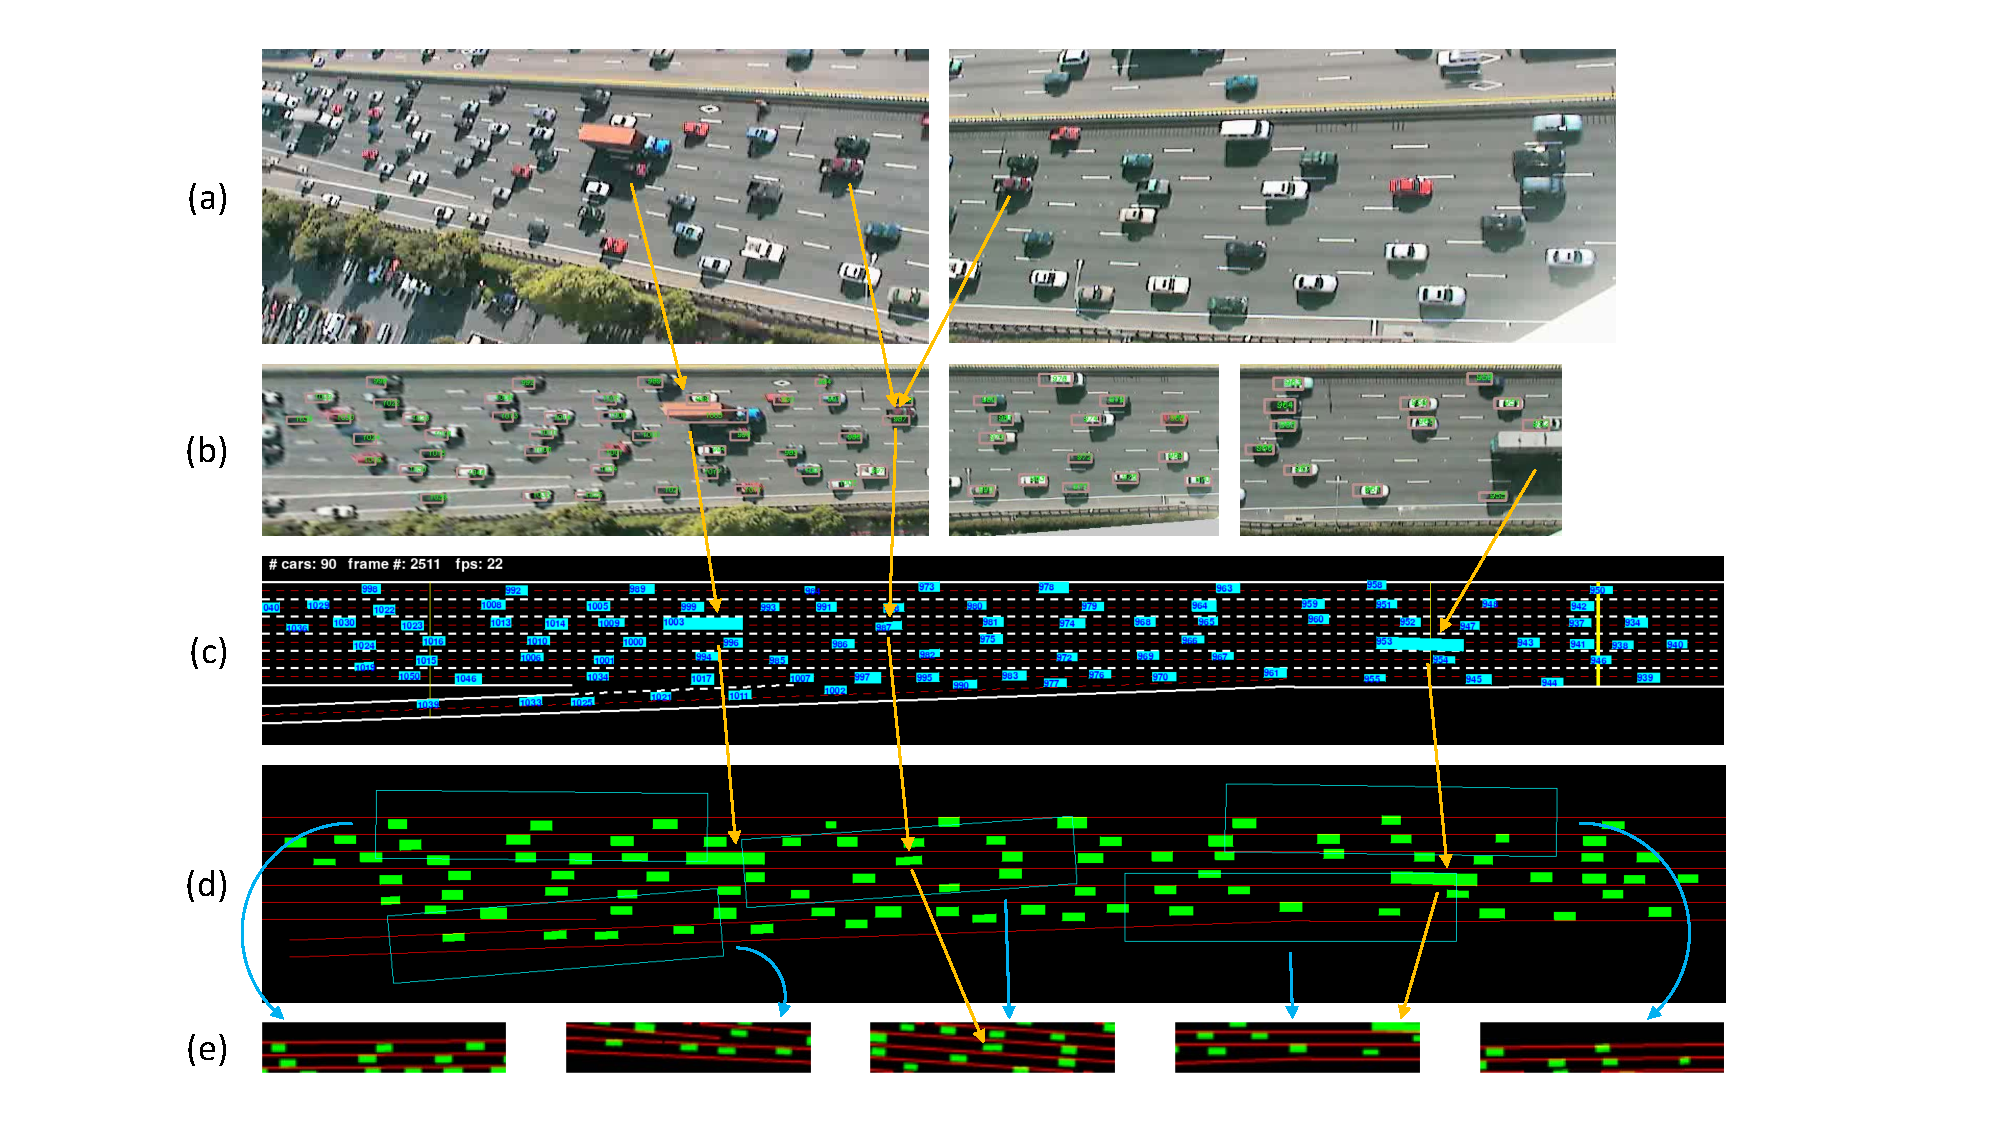
\includegraphics[width=\textwidth]{figures/driving/I-80.pdf}
  \caption{
    Preprocessing pipeline for the NGSIM-I80 data set.
    Orange arrows show same vehicles across stages.
    Blue arrows show corresponding extracted context state.
    (a) Snapshots from two of the seven cameras.
    (b) View point transformation, car localisation and tracking.
    (c) Every vehicle in the simulator is initialised with starting position, initial velocity, dimensions, and ID number.
    %    A longitudinal and transverse inter-vehicle linear proximity cost is computed, which is maximum in case of collision and goes to zero if vehicles are sufficiently spaced.
    (d) Context states are extracted from rectangular regions surrounding each vehicle.
    (e) Five examples of context states extracted at the previous stage.
    Notice how vehicles oriented slightly to the left (2nd and 3rd examples) have lane markings rotated to the right.
  }
\label{I-80}
\end{figure}


\textbf{State representation}:
Our state representation consists of two components: an image representing the neighborhood of the car, and a vector representing its current position and velocity.
For the images, we rendered images centered around each car which encoded both the lane emplacements and the locations of other cars.
Each image has 3 channels: the first (red) encodes the lane markings, the second (green) encodes the locations of neighboring cars, which are represented as rectangles reflecting the dimensions of each car, and the third channel (blue) represents the ego car, also scaled to the correct dimensions.
All images have dimensions $3 \times 117 \times 24$, and are denoted by $i_t$.
\footnote{Another possibility would have been to construct feature vectors directly containing the exact coordinates of neighboring cars, however this presents several difficulties.
First, cars can enter and exit the neighborhood, and so the feature vector representing the neighboring cars would either have to be dynamically resized or padded with placeholder values.
Second, this representation would not be permutation-invariant, and it is unclear where to place a new car entering the frame.
Third, encoding the lane information in vector form would require a parametric representation of the lanes, which is more complicated.
Using images representations naturally avoids all of these difficulties.}
Two examples are shown in Figure \ref{cost}.
We also computed vectors $u_t = (p_t, \Delta p_t)$, where $p_t = (x_t, y_t)$ is the position at time $t$ and $\Delta p_t = (x_{t+1} - x_t, y_{t+1} - y_t)$ is the velocity.


\begin{figure}
  \centering
  \subfigure[19.8 km/h]{
  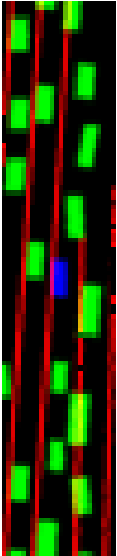
\includegraphics[height=0.3\textheight]{figures/driving/image_198-crop.pdf}
  
\includegraphics[height=0.3\textheight]{figures/driving/mask_198-crop.pdf}
  }
  \hspace{15mm}
  \subfigure[50.3 km/h]{
  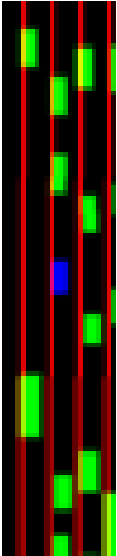
\includegraphics[height=0.3\textheight]{figures/driving/image_503-crop.pdf}
  
\includegraphics[height=0.3\textheight]{figures/driving/mask_503-crop.pdf}
  }
  \caption{Image state representations and proximity cost masks for cars going at different speeds. The higher the speed, the longer the safety distance required to maintain low cost.}
\label{cost}
\end{figure}







%Every vehicle in the simulator is initialised with starting position $\bm{p} = (x, y)$, initial velocity $v \bm{d}$ (where $v$ represents the speed and $\bm{d}$ the direction versor), correct dimensions, and identification (ID) number.
%At every time step $\Delta t = 0.1\,\text{s}$, we use the tracked trajectories (previously smoothed with a $1.5\,\text{s}$ running average) and a simplified kinematic model of a car to compute the agent actions $(a, b)$, corresponding to acceleration and tangential deviation.
%Therefore, the vehicle internal state is updated with: $\bm{p} \gets \bm{p} + v \bm{d} \Delta t$, $v \gets v + a \Delta t$, $\bm{d} \gets \bm{d} + v b \bm{d}_\perp \Delta t$, and $\bm{d} \gets \bm{d} / \lVert \bm{d} \rVert$.
%A longitudinal and transverse inter-vehicle linear proximity cost is computed, which is maximum in case of collision and goes to zero if vehicles are sufficiently spaced.
%Finally, the vehicles are drawn onto the screen canvas and displayed with their corresponding ID number.
%\textbf{(d)} Lanes and vehicles are also drawn on a secondary canvas, from which the context states are extracted.
%Rectangular regions around each vehicle --- oriented according to $\bm{d}$, of length corresponding to twice the space travelled in $1\,\text{s}$ at $130\,\text{km/h}$, of width equal four times the lane width --- scaled by a $0.5$ factor constitute the context states.
%    At this stage, the lane-crossing cost is computed using a modified morphological distance transform between each vehicle and the lane channel.



\textbf{Action representation}: Each action vector $a_t$ consists of two components: an acceleration (which can be positive or negative) which reflects the change in speed, and a change in angle.
The acceleration at a given time step is computed by taking the difference between two consecutive speeds, while the change in angle is computed by projecting the change in speed along its orthogonal direction:

\begin{align*}
  \Delta \mbox{speed} &= \| \Delta p_{t+1} \|_2 - \| \Delta p_t \|_2 \\
  \Delta \mbox{angle} &= (\Delta p_{t+1} - \Delta p_t)^\top (\Delta p_t)_\perp / \| \Delta p_t \|_2  \\
  a_t &= (\Delta \mbox{speed}, \Delta \mbox{angle}) \\
\end{align*}




\textbf{Cost}: Our cost function has two terms: a proximity cost and a lane cost. The proximity cost reflects how close the ego car is to neighboring cars, and is computed using a mask in pixel space whose width is equal to the width of a lane and whose height depends on the speed of the car. Two examples are shown in Figure \ref{cost}.
This mask is pointwise multiplied with the green channel, and the maximum value is taken to produce a scalar cost.
The lane cost uses a similar mask fixed to the size of the car, and is similarly multiplied with the red channel, thus measuring the car's overlap with the lane.
Both of these operations are differentiable so that we can backpropagate gradients with respect to these costs through images predicted by a forward model.

This preprocessing yields a set of state-action pairs $(s_t, a_t)$ (with $s_t=(i_t, u_t)$) for each car, which constitute the dataset we used for training our prediction model.
We then use the cost function to optimize action sequences at planning time, using different methods which we describe in Section \ref{planning-methods}.

We now describe how we adapted this dataset to be used as an environment to evaluate planning methods.
Building an environment for evaluating policies for autonomous driving is not obvious as it suffers from a cold-start problem.
Precisely measuring the performance of a given driving policy would require it to be evaluated in an environment where all other cars follow policies which accurately reflect human behavior.
This involves reacting appropriately both to other cars in the environment as well as the car being controlled by the policy being evaluated.
However, constructing such an environment is not possible as it would require us to already have access to a policy which drives as humans do, which in some sense is our goal in the first place. One could hand-code a driving policy to control the other cars in the environment, however is it not clear how to do so in a way which accurately reflects the diverse and often unpredictable nature of human driving.

We adopt a different approach where we let all other cars in the environment follow their trajectories in the dataset, while controlling one car with the policy we seek to evaluate.
The trajectory of the controlled car is updated as a function of the actions output by the policy, while the trajectories of the other cars remain fixed.
If the controlled car collides with another car, this is recorded and the episode ends.
This approach has the advantage that all other cars in the environment maintain behavior which is close to human-like.
The one difference with true human behavior is that the other cars do not react to the car being controlled or try to avoid it, which may cause crashes which would not occur in real life.
The driving task is thus possibly made more challenging than in a true environment, which we believe is preferable to using a hand-coded policy.
The interface is set up the same way as environments in OpenAI Gym \citep{OpenAIBaselines}, and can be accessed with a few lines of Python code, as shown in Figure \ref{interface}.




\begin{figure}
  \centering
  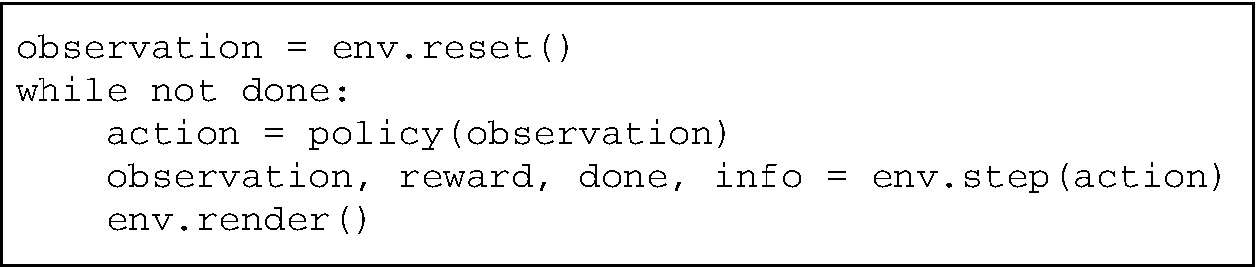
\includegraphics[width=0.8\textwidth]{figures/driving/traffic_gym_code-crop.pdf}
  \caption{NGSIM planning environment.}
\label{interface}
\end{figure}







%This data set reflects complex interactions between a large number of agents (in this case vehicle drivers), leading to a challenging prediction problem which can be useful for evaluating new methods more generally.
%Current video prediction data sets used in the literature to evaluate stochastic prediction models consist of Synthetic Moving MNIST (SM-NIST) digits \citep{Denton2018}, BAIR robot manipulation videos \citep{Ebert17}, or videos of human movements \citep{Denton2018, Babaeizadeh2018}.
%These have the advantage of being able to evaluate specific model capabilities in a controlled setting, and have applications in robotics.
%However, they also have relatively few degrees of freedom: \emph{e.g.}\ the SM-MNIST data set latent variables are two-dimensional (vertical and horizontal random velocities are picked), while the major factors of variation within the BAIR robot data set can also be captured with two dimensions \textcolor{red}{(\emph{i.e.}\ the position or velocity of the robot arm, which we demonstrate in our experiments)}.
%In contrast, the NGSIM I-80 data set has a relatively large number of cars per context image, as shown in \cref{car-statistics}, with each car having multiple degrees of freedom.
%We therefore believe this prediction tasks offers unique features which complement other data sets used in the literature.








\section{Stochastic Forward Model}

We next describe our stochastic forward model, starting with a general version and followed by a specific instantiation which uses the state representations described in the previous section.
%We first describe the general version of the model, followed by the specific instantiation for this dataset.
Our model, which we call the Target Encoding Network (TEN), can be viewed as a conditional autoencoder paired with a non-parametric sampling procedure.
The architecture consists of three neural networks: an encoder $f_\text{enc}$, a decoder $f_\text{dec}$, and a latent variable network $f_\phi$.
For each input $s_{1:t}$ (i.e. a sequence of $t$ consecutive states), action $a_t$, and  target $s_{t+1}$ (i.e. the following state), the update equations are given by:
%
\begin{align}
  \label{eq:update-eqn}
  z_t &= f_\phi(s_{1:t}, s_{t+1}) \cdot u, u \in \{0, 1\} \sim \mathcal{B}(p) \\
  \tilde{s}_{t+1} &= f_\text{dec}(f_\text{enc}(s_{1:t}), a_t, z_t) = f_\theta(s_{1:t}, a_t, z_t)
\end{align}
%
where $z_t$ is the latent variable vector associated to the input $s_{1:t}$, $\tilde{s}_{t + 1}$ is the predicted target state, and $\mathcal{B}(p)$ is a Bernoulli random variable with probability $p$.
All networks are trained by gradient descent to optimize the following objective:
%
\begin{align}
%  \ell(\tilde{s}_{t+1}, s_{t+1}) &= \lVert \tilde{s}_{t+1} - s_{t+1} \rVert_2^2 \\
  \ell(\tilde{s}_{t+1}, s_{t+1}) = \ell(f_\theta(s_{1:t}, a_t, f_\phi(s_{1:t}, s_{t+1}) \cdot u), s_{t+1})
  \label{ten-loss}
\end{align}


\begin{figure}[t!]
    \centering
    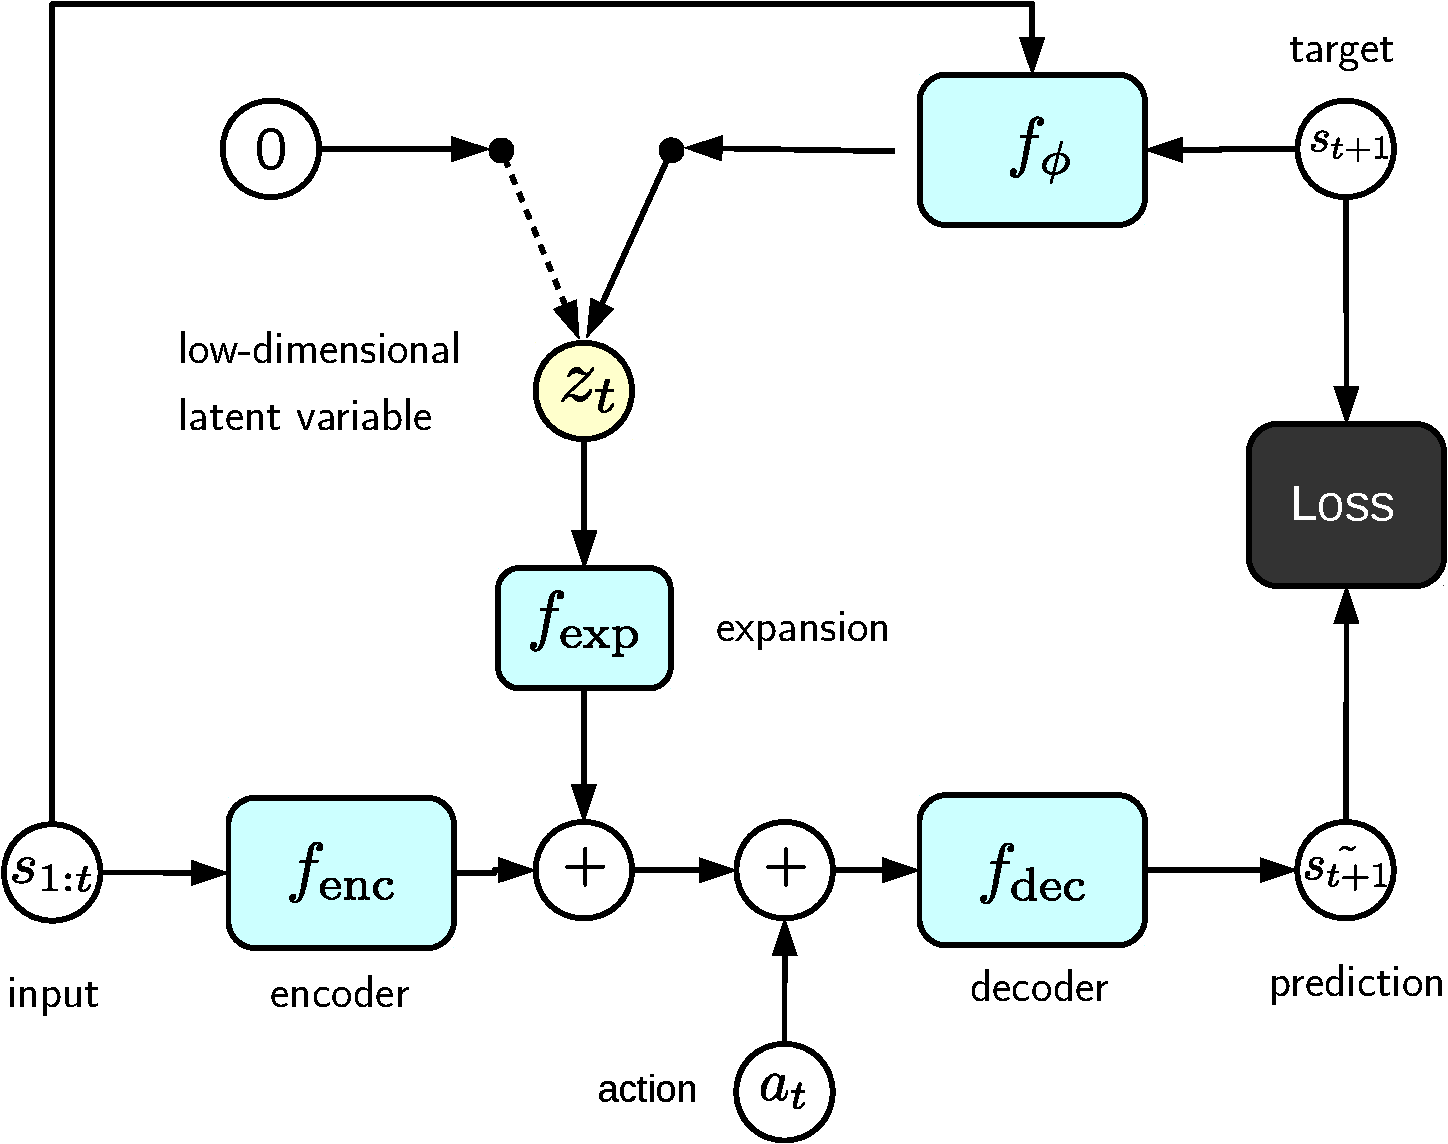
\includegraphics[width=0.7\textwidth]{figures/driving/ten_train-crop.pdf} \\
    \label{ten}
    \caption{Target Encoding Network}
\end{figure}


where $\ell$ is a per-sample loss appropriate to the task at hand. Note in particular that no sampling of the latent variable or reparamaterization is done at training time.
In standard autoencoders, some mechanism is used to limit the information content of the latent representation to avoid learning trivial mappings and thus encourage the model to learn good representations.
In the conditional case we are considering, we also need such a mechanism to prevent the network from simply reconstructing $s_{t+1}$ from $z_t$ while ignoring the input $s_{1:t}$ and action $a_t$.
This is accomplished by setting the latent vector $z_t$ to zero with some probability $1 - p$ at every training iteration.
This setting encourages the network to continue to extract as much information as possible from the input $s_{1:t}$ and action $a_t$, rather than simply trying to reconstruct the target, and only use the true target $s_{t+1}$ to reconstruct what cannot be predicted from the input.
In our experiments, we train with $p = 0$ for an initial fixed number of iterations, which corresponds to purely deterministic training, after which we increase $p$ to incorporate the latent variables encoded from the targets.

A second key point is that the dimension of the latent variable $z$ is much lower than the dimension of the state $s$.
This has two benefits: first, it can further help limit the information content and prevent trivial reconstructions of the targets.
Second, it allows us to use non-parametric estimates of the distribution over latent variables using a reasonable number of points, which we detail next.
A transformation $f_\text{exp}$ transforms this low-dimensional latent variable to be the same size as the hidden representation, after which it is combined via addition.
Note that in the case of a linear transformation, this simply corresponds to combining the latent variable and hidden state via concatenation.


After the model is trained, we obtain a non-parametric estimate of the distribution over latent vectors by extracting a large collection of $z$ vectors from the training set, which we refer to as $\mathcal{Z} = \{ z_t \} = \{ f_\phi(s_{1:t}, s_{t+1}) \}$.
For an unseen input $s_{1:t}'$ and action $a_t'$, we simply sample some $z \sim \mathcal{Z}$ uniformly at random, and feed it into the forward model to obtain a future prediction $f_\theta(s_{1:t}', a_t', z)$.



Other works have proposed models for stochastic prediction based on Variational Autoencoders (VAEs) \citep{VAE}.
These models assume a parametric prior over the latent variables, and include an additional term in the loss function to enforce a match between the prior and the distribution over latent variables produced by a posterior network, which plays a similar role to the $f_\phi$ network here.
This match between distributions is usually measured using the KL divergence.
At test time, latent variables are then sampled from this parametric prior.
Our model can also be viewed within the VAE framework as having a uniform categorical prior over $z$ vectors extracted from each sample in the training set (where a sample is a pair $(s_{1:t}, s_{t+1})$), and a posterior distribution which is a one-hot categorical distribution at the current training sample.
More specifically, let $M$ denote the number of samples in the training set, let $p = (\frac{1}{M}, ..., \frac{1}{M})$ denote the prior and $q=(0, ..., 0, 1, 0, ..., 0)$ denote the posterior. The KL divergence between prior and posterior is then:

\begin{align*}
  D_{KL}(q||p) &= \sum_{i=1}^M q_i \mbox{ log } \frac{q_i}{p_i} \\
  &= 1 \cdot \mbox{ log } \frac{1}{\frac{1}{M}} \\
  &= \mbox{ log } M
\end{align*}

Note that this term depends only on the size of the dataset and not the output of the posterior network $f_\phi$, and therefore has zero gradient and does not affect optimization, hence we recover the loss in Equation \ref{ten-loss}.
%If there is a single dataset sample, the posterior is matched with the prior and the KL divergence vanishes, achieving the variational lower bound.
The main motivation behind our model is its ease of training and lack of sensitive hyperparameters governing the tradeoff between prediction loss and prior matching.
We found that with sufficient tuning, it was possible to train VAEs to obtain similar performance as our model, and we compare planning performance of the two models in our experiments.

\begin{figure}[t!]
    \centering
    \subfigure[$f_{enc}$]{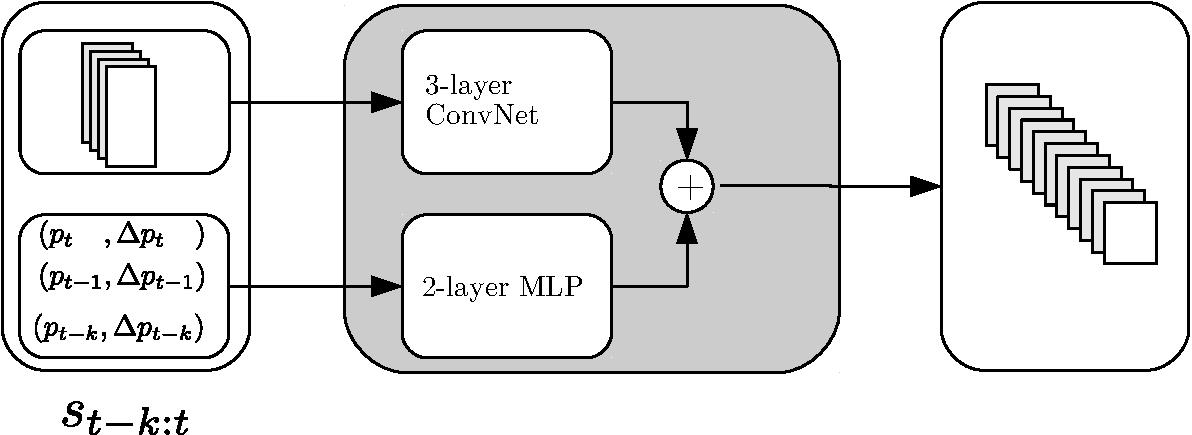
\includegraphics[width=0.45\textwidth]{figures/driving/f_enc-crop.pdf}} \\
    \subfigure[$f_{dec}$]{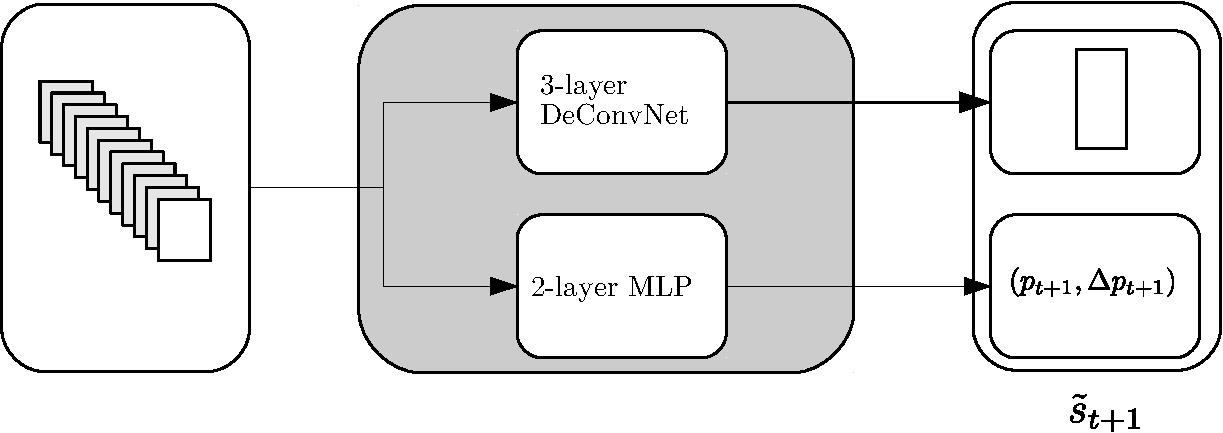
\includegraphics[width=0.45\textwidth]{figures/driving/f_dec-crop.pdf}} \\
    \subfigure[$f_\phi$]{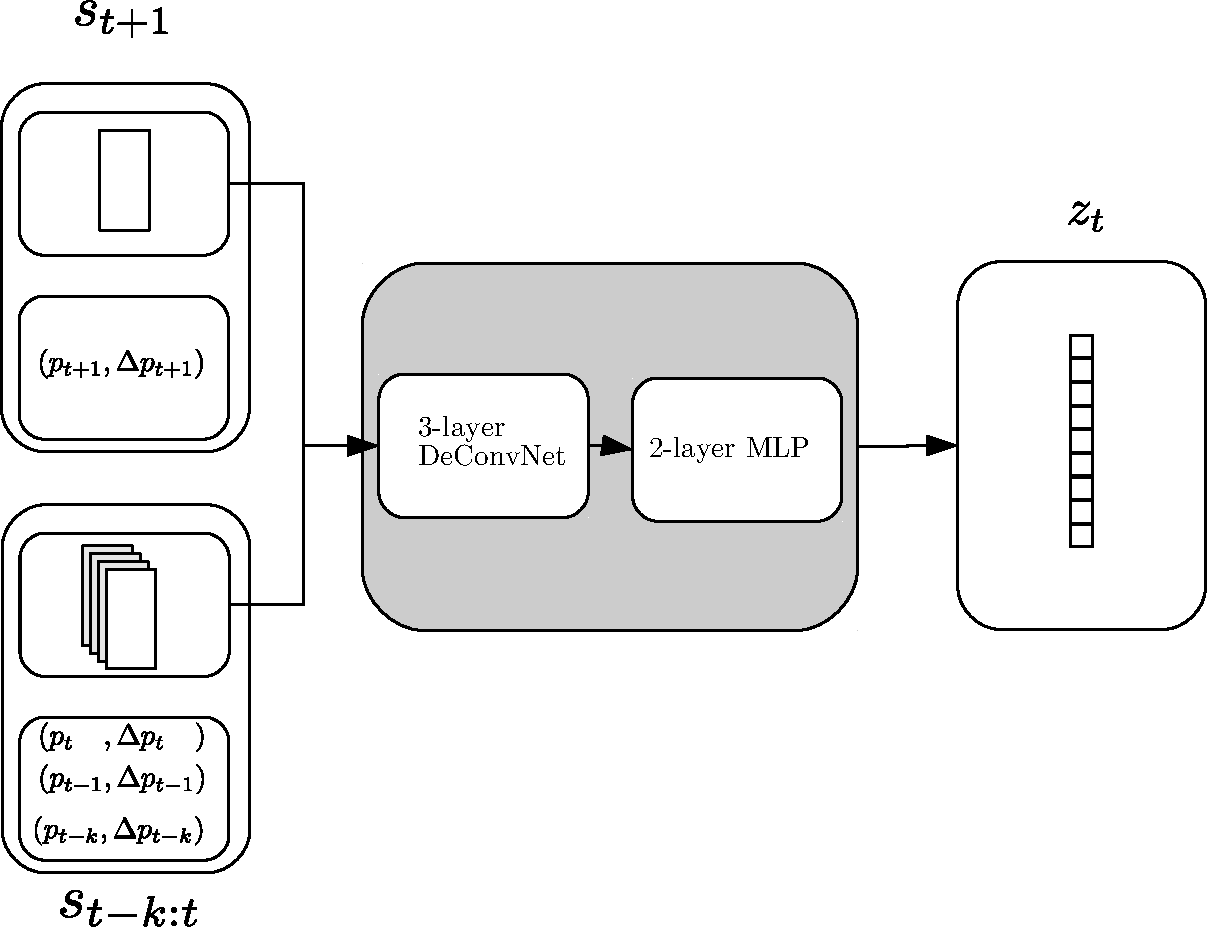
\includegraphics[width=0.45\textwidth]{figures/driving/f_phi-crop.pdf}} \\
    \caption{Individual components of the stochastic prediction model.}
\end{figure}
\label{model-components}


We now describe the specific instantiation used in this dataset, shown in Figure \ref{model-components}. At every time step, it takes as input the concatenation of 20 previous states, each of which consists of a context image $i_t$ and a 4-dimensional vector $u_t$ encoding the car's position and velocity, and a 2-dimensional action $a_t$ encoding the car's acceleration and change in steering angle.
The images $i_{t-20}, ..., i_t$ are run through a 3-layer convolutional network, and the other inputs are run through 2-layer fully connected networks, whose final layers contain the same number of hidden units as the number of elements in the output of the convolutional network. The outputs of the fully-connected layers are combined with that of the convolutional network by addition.
The result is then run through a deconvolutional network, which produces a prediction for the next image $i_{t+1}$, and a fully-connected network which produces a prediction for the next state vector $u_{t+1}$.
The per-timestep prediction loss which the model optimizes in Equation \ref{ten-loss} is given by:

  \begin{equation}
    \ell(\tilde{s}_t, s_t) = \|\tilde{i}_t - i_t \|_2^2 + \| \tilde{u}_t - u_t \|_2^2
  \end{equation}
















  \section{Planning Approaches}
  \label{planning-methods}

  We now describe different planning approaches using our stochastic forward model, with diagrams shown in Figure \ref{planning-methods}.
  All methods except model-predictive control make use of a policy network which has the same architecture.
  It consists of an encoder with an identical architecture as $f_{enc}$ used in the forward model (which also takes 20 consecutive states as input), followed by a 3-layer fully connected network which outputs a 2-D mean and variance $(\mu, \sigma)$ of a diagonal Gaussian over actions.

  Two of the planning methods optimize a cost function $C$, which is a combination of the proximity and lane costs we described previously, as well as an epistemic uncertainty cost which we describe in the next section. For now, we can treat the cost as a scalar-valued differentiable function of a predicted state.


\begin{figure*}[ht!]
    \centering
    \subfigure[Stochastic Model-Based Imitation Learning (SMBIL)]{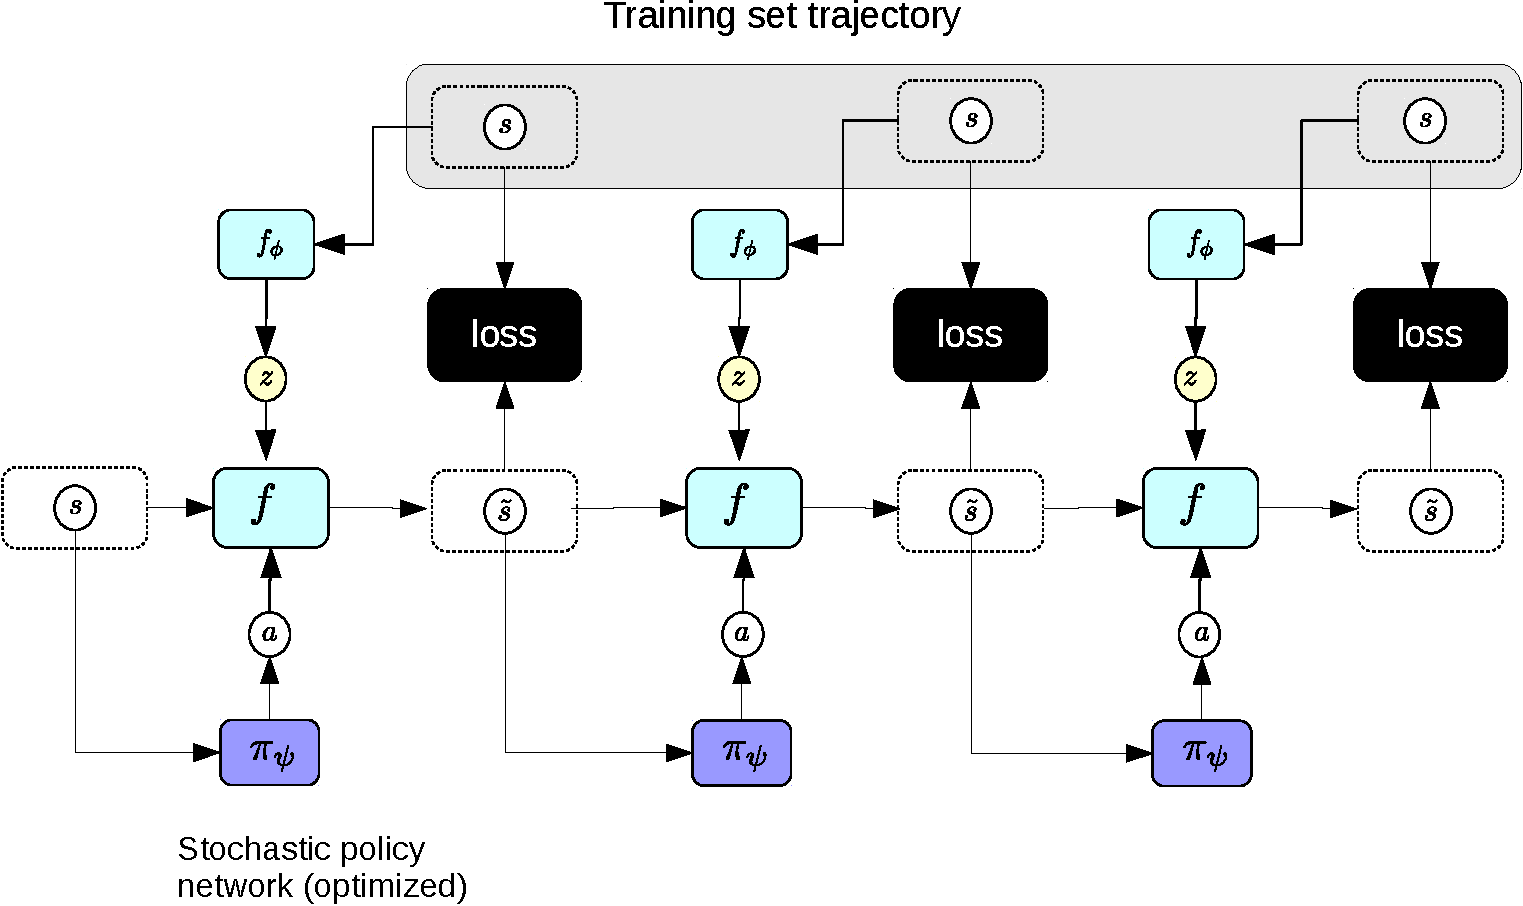
\includegraphics[width=0.5\textwidth]{figures/driving/smbil-crop.pdf}} \\
    \subfigure[Stochastic Value Gradients (SVG)]{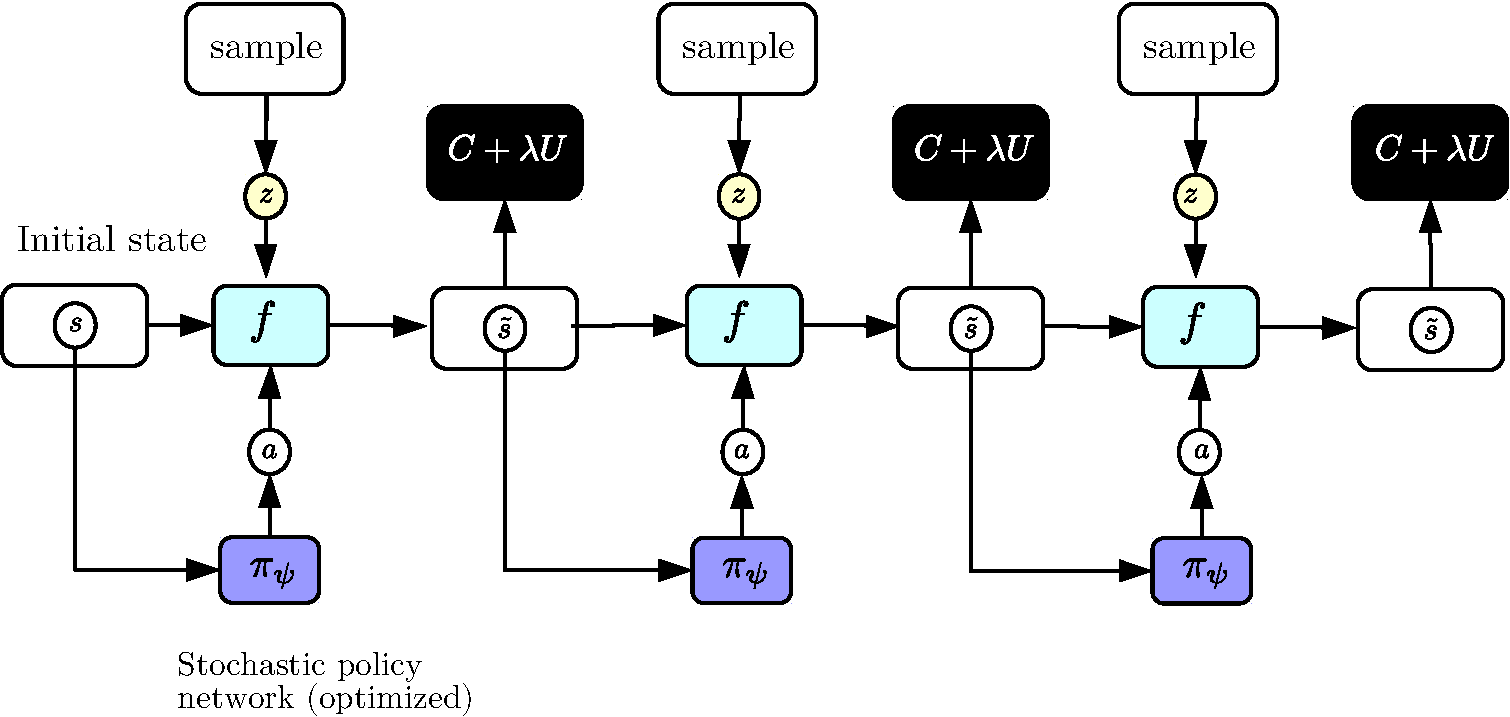
\includegraphics[width=0.5\textwidth]{figures/driving/svg-crop.pdf}} \\
    \subfigure[Stochastic Model-Predictive Control (SMPC)]{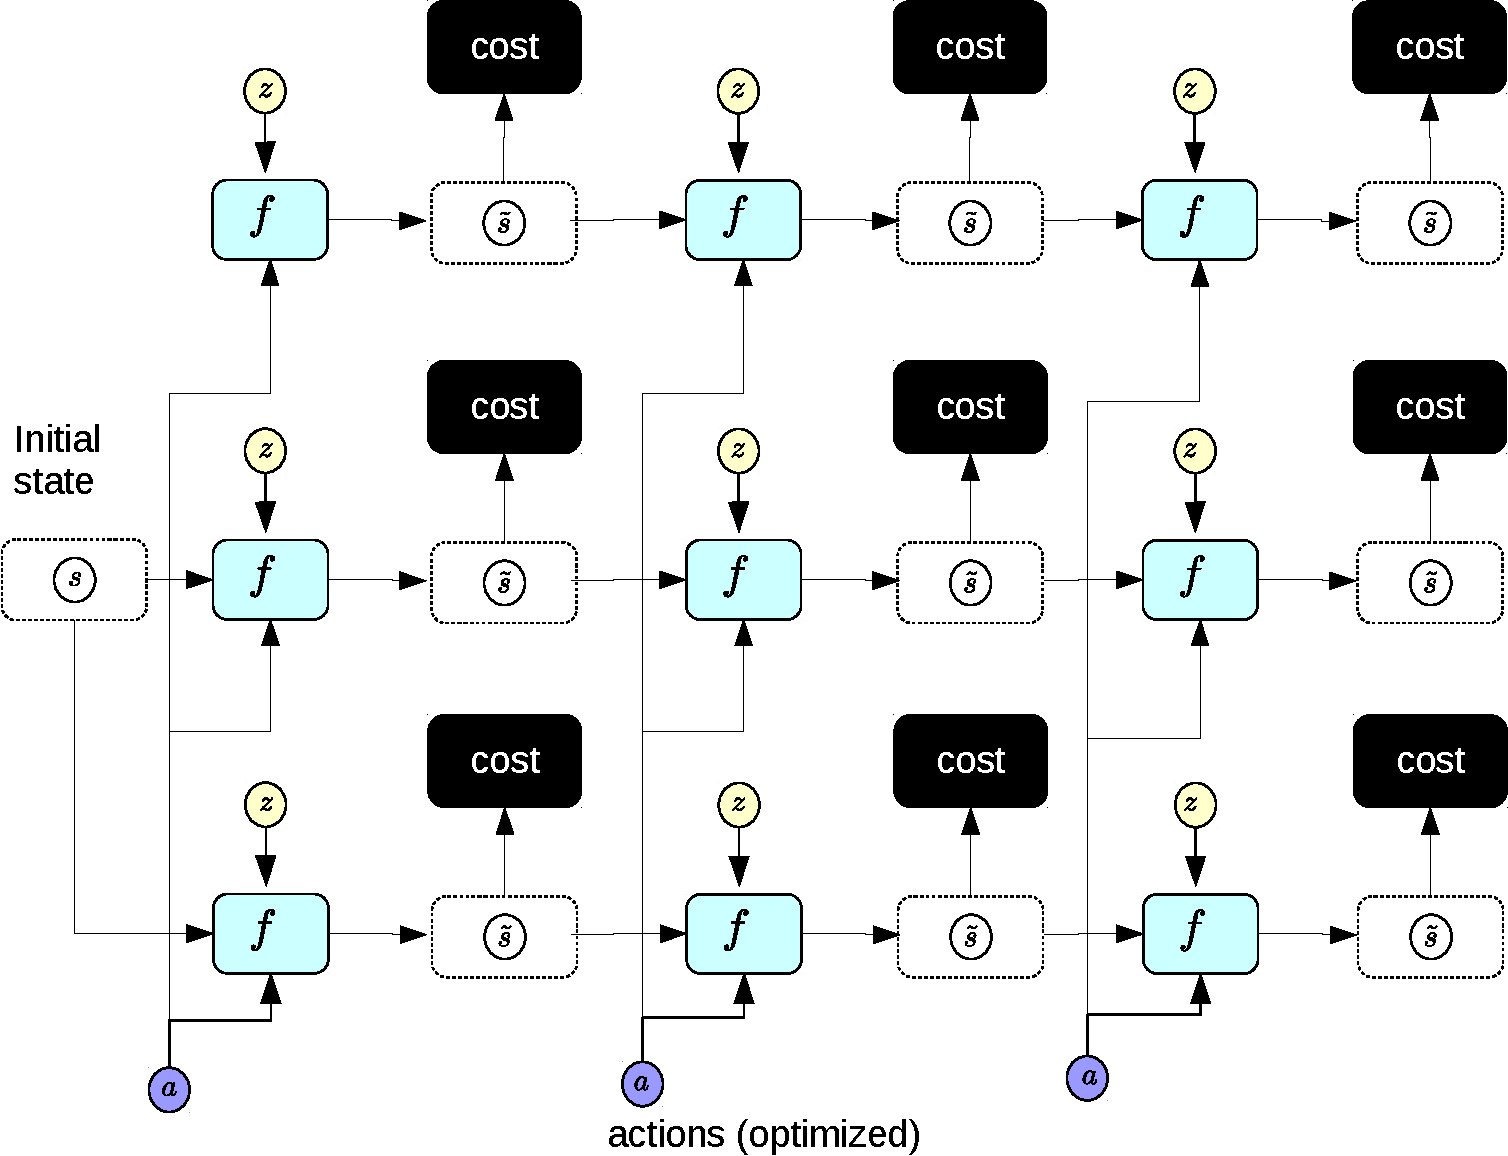
\includegraphics[width=0.5\textwidth]{figures/driving/mpc-crop.pdf}} \\
    \label{planning-methods}
    \caption{Planning Methods. SMBIL minimizes the distance between training set trajectories and trajectories predicted by the forward model under the current policy network, using latent variables inferred from the training trajectory. The other methods optimize actions or a policy network to minimize the cost predicted by the forward model, using randomly sampled sequences of latent variables.}
\end{figure*}



  \subsection{Single-Step Imitation Learning}


  The simplest approach to learning a policy from observational data is imitation learning \citep{Pomerleau91}, where a network is trained to predict expert actions from states. Here, we give the network a concatenation of 20 states $s_{1:t}$ as input and train it to minimize the negative log-likelihood of the true action observed in the dataset under the parameters of the distribution output by the model:

    \begin{align*}
    \underset{\psi}{\mbox{ argmin }} \Big[ -\mbox{ log } \mathcal{N}(a_{t+1} | \mu, \sigma) \Big],  \mbox{ such that: } (\mu, \sigma) = \pi_\psi(s_{1:t}) \\
  \end{align*}

  \subsection{Stochastic Model-Based Imitation Learning (SMBIL)}

  We also experimented with a variant of imitation learning using the learned stochastic model, which we found performed better than the standard version. One issue with imitation learning is that errors can accumulate quickly, leading to divergence from the states seen during training.
  One cause may be that the model is simply minimizing the $\ell_2$ loss in action space, which may not correspond to minimizing distances in trajectory space.
  Consider the following example where an agent is walking exactly along the side of a cliff, and must output an action which represents its angle.
  To the left is a drop, and to the right is solid ground.
  Say the expert action is to go straight, i.e. $a_{t+1} = 0$. Now consider two possible actions predicted by the network, $\tilde{a}_{t+1} = -\epsilon$ (slight left) and $\tilde{a}_{t+1} = +\epsilon$ (slight right).
  Both of these actions incur the same $\ell_2$ cost of $\epsilon$, but have very different consequences. If the agent moves slightly away from the expert action on the left side, they fall off the cliff, which causes a large deviation of their subsequent states from the expert states. If they move slightly to the right however, they stay on solid ground and their subsequent states remain close to the expert states.

  As an alternative, we experimented with training a policy to match expert \textit{trajectories}, rather than actions.
  We do this by unrolling the forward model for multiple timesteps, outputting actions by the policy network using the model predictions, and minimizing the error between the final trajectory output by the forward model and the expert trajectory observed in the dataset.
%  This is illustrated in Figure \ref{mbil-diagram}.
  The motivation here is that if the policy network outputs an action which causes small divergence from the target trajectory at the next timestep, but large divergences later on, it will receive gradients from these larger errors backpropagated through the unrolled forward model.

    \begin{align*}
    \underset{\psi}{\mbox{ argmin }} \Big[ \sum_{i=1}^{T} \ell(s_{t+i}, \tilde{s}_{t+1}) \Big],  \mbox{ such that: }
    \begin{cases}
      \tilde{s}_t = s_t \\
      z_{t+i} = f_\phi(\tilde{s}_{t+i-1}, \tilde{s}_{t+i}) \\
      \tilde{a}_{t+i} = \pi_\psi(\tilde{s}_{t+i-1}) \\
      \tilde{s}_{t+i} = f(\tilde{s}_{t+i-1}, \tilde{a}_{t+i}, z_{t+i}) \\
      \end{cases}
  \end{align*}


%  \begin{figure}[t]
%\centering
%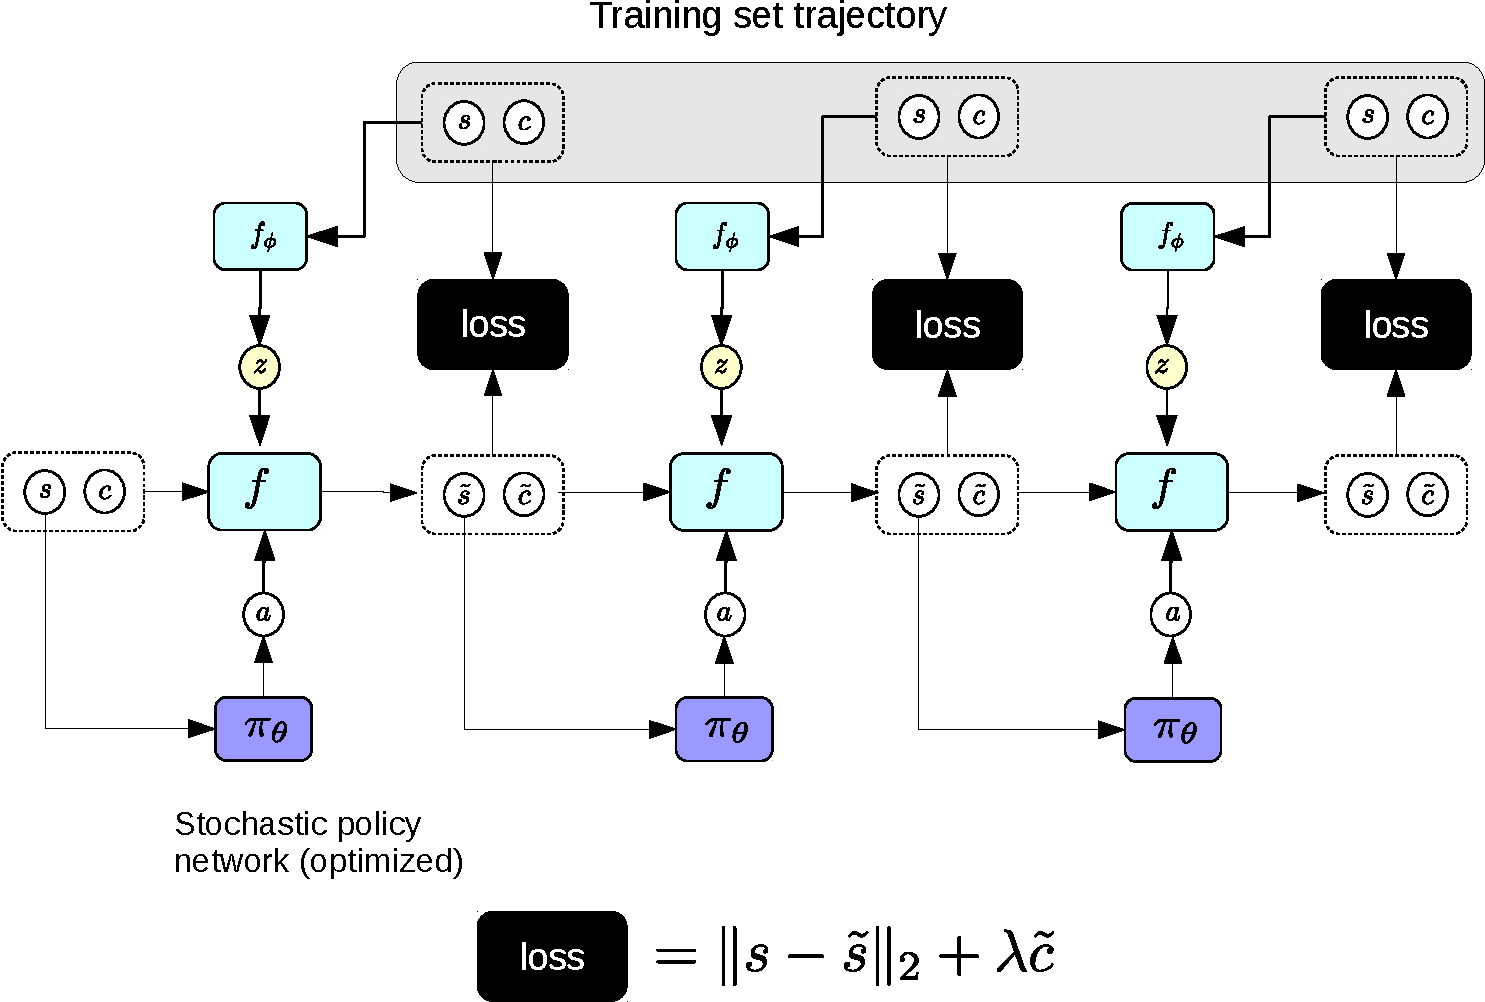
\includegraphics[width=0.95\textwidth]{figures/driving/mbil.pdf}
%\caption{Stochastic Model-Based Imitation Learning. The forward model is unrolled for several time steps and latent variables are inferred from the training sequence. Keeping these fixed, the policy network is optimized to produce actions such that the training trajectory is matched.}
%\label{mbil-diagram}
%\end{figure}


    \subsection{Stochastic Model-Predictive Control (SMPC)}
    \label{MPC}

  We also evaluated a receding-horizon model-predictive controller (MPC). At each time step, we optimize a sequence of actions over the next $T$ timesteps under the forward model and execute the first one.
  Since the model is stochastic, we sample $K$ different sequences of latent variables and optimize the same action sequence averaged over all of them.
  This requires solving the following optimization problem at each time step $t$:

  \begin{align*}
    \underset{a_t, ..., a_{t+T}}{\mbox{ argmin }} \Big[ \frac{1}{K} \sum_{k=1}^K \sum_{i=1}^{T} C(s_{t+i}^k) \Big],  \mbox{ such that: }
    \begin{cases}
      z_{t+i}^k \sim p(z) \\
      \tilde{s}_t^k = s_t  \\
      \tilde{s}_{t+i}^k = f(\tilde{s}_{t+i-1}^k, a_{t+i}, z_{t+i}^k) \\
      \end{cases}
  \end{align*}

  We solve this optimization problem by performing $N$ steps of gradient descent over the sequence of actions $a_t, ..., a_{t+T}$, during which all the sampled sequences of latent variables are held fixed.
  Intuitively, this optimization problem can be interpreted as follows. We draw $K$ different sequences of latent variables, which represent $K$ different ways in which the future can unfold.
  We then optimize a single action sequence, to minimize the predicted costs averaged over each of these possible futures.
  We thus hope to obtain an action sequence which performs well in many scenarios.

  This procedure is unfortunately expensive: it requires a total of $K \times N \times T$ model evaluations. Although the model evaluations corresponding to $K$ different futures can be done in parallel on the GPU, evaluations at different time steps and over different optimization iterations must be done sequentially.
  We found that maintaining a buffer of previously planned actions allowed us to get better performance with a relatively small number of iterations; this was proposed in \citep{Ohtsuka04}.
  Specifically, at every time step we plan for the next $T$ actions, but only execute the first even though the subsequent ones may be reasonable.
  We therefore initialize the action sequence to be optimized at the next timestep with the result of the action sequence optimized at the previous time step, shifted by one:

  \begin{equation}
    (a_t, a_{t+1}, a_{t+2}, ..., a_{T-1}, a_T) \leftarrow (a_{t+1}, a_{t+2}, ..., a_{T-1}, a_T, \mathbf{0})
  \end{equation}


  \subsection{Stochastic Value Gradients (SVG)}

  The last approach which we explored was designed to train a policy network using the learned stochastic forward model, using the framework of Stochastic Value Gradients \citep{SVG}.
  We first randomly sample an initial input state $s_t$ from the training set, sample a sequence of latent variables $z$ to represent a future scenario, and then optimize a paramaterized policy network $\pi_\psi$ to minimize the cost predicted by the forward model conditioned on this sequence of latent variables.

    \begin{align*}
    \underset{\psi}{\mbox{ argmin }} \Big[ \sum_{i=1}^{T} C(s_{t+i}) \Big],  \mbox{ such that: }
    \begin{cases}
      z_{t+i} \sim p(z) \\
      \tilde{a}_{t+i} = \pi_\psi(s_{t+i-1}) \\
      \tilde{s}_{t+i} = f(\tilde{s}_{t+i-1}, \tilde{a}_{t+i}, z_{t+i}) \\
      \end{cases}
    \end{align*}

    Our approach differs somewhat from the setup of \citep{SVG}, who used latent variables inferred from ground truth trajectories as a means to compensate for model errors. We did not find this to be a problem, possibly because we trained the forward model to make 20-step predictions, whereas they trained the forward model to make single-step predictions.






    \section{Differentiable Epistemic Uncertainty Cost}

    We propose to augment the proximity and lane costs described in Section \ref{i80-dataset-prep} with an additional term which penalizes the uncertainty of the forward model, calculated using dropout, and use derivatives of this cost for planning.
    Dropout \citep{Dropout2012, Dropout2014} consists of randomly setting hidden units in a neural network to zero with some probability, and has been shown to substantially reduce overfitting.
%    The original work proposes an loose connection with model ensembling, by viewing the same model with different dropout masks as different models in an ensemble.
    The work of \citep{Gal16} showed that a neural network trained with dropout is mathematically equivalent to an approximation of a probabilistic deep Gaussian Process model, which includes uncertainty estimates.
    A key result of this is that estimates of the neural network's epistemic uncertainty can be obtained by calculating the variance of an output given the same input over multiple dropout masks.
    More precisely, let $f_{\theta_1}, ..., f_{\theta_K}$ be the same model $f_\theta$ with $K$ different dropout masks, and for some input $x$, let $y_k=f_{\theta_k}(x)$.
    The uncertainty of the original model about a given prediction $y=f_\theta(x)$ is given by the covariance matrix of the outputs under different dropout masks (up to some constants):

    \begin{align}
      \mbox{Cov}[y_1, ..., y_K] = \frac{1}{K} \Big[ \sum_{k=1}^K y_k y_k^\top \Big] - \Big[ \frac{1}{K}\sum_{k=1}^K y_k \Big] \Big[\frac{1}{K}\sum_{k=1}^K y_k)\Big]^\top
    \end{align}

    We note that this uncertainty estimate is the composition of differentiable functions: each of the models with different dropout masks is differentiable, as is the covariance operator.
    Furthermore, we can summarize the covariance matrix by taking its trace (which is equal to the sum of its eigenvalues, or equivalently the sum of the variances of the outputs across each dimension), which provides a scalar estimate of uncertainty which is also differentiable with respect to the inputs.
    This allows us to obtain gradients of the inputs with respect to this measure of epistemic uncertainty, which gives us directions in input space which would make the model more certain.

    In the context of our stochastic forward model, we define an epistemic uncertainty estimate as follows:

    \begin{align*}
      \Omega(s_{1:t}, a_t, z_t) &= \mbox{tr} \Big[ \mbox{Cov} [\{ f_{\theta_k}(s_{1:t}, a_t, z_t) \}_{k=1}^K] \Big] \\
      %      &= \frac{1}{K} \Big[ \| f_{\theta_k}(s_{1:t}, a_t, z_t) - \sum_{k=1}^K f_{\theta_k}(s_{1:t}, a_t, z_t) \|_2^2 \Big]
      &= \sum_{j=1}^D \mbox{Var}(\{ f_{\theta_k}(s_{1:t}, a_t, z_t)_j \}_{k=1}^K)
    \end{align*}

    where $D$ is the dimensionality of the output. Minimizing this quantity with respect to actions encourages a planning algorithm or policy network to produce actions which, when plugged into the forward model, will produce predictions which the model is confident about.
%    We observed, however, that this quantity varies for different rollout lengths and for different output modalities of our forward model (for example, images and state vectors).
%    In particular, the uncertainty increases as the forward model is rolled out for more time steps.
    To compensate for differences in baseline uncertainty across different modalities or rollout lengths, for each modality we estimate the empirical mean and variance of $\Omega$ for every rollout length $t$ of the forward model over the training set, to obtain $\mu_{\Omega}^t$ and $\sigma_{\Omega}^t$. We then define our epistemic uncertainty cost as follows:

    \begin{align}
      C_U(s_{1:t}, a_t, z_t) = \Big [ \frac{\Omega(s_{1:t}, a_t, z_t) - \mu_\Omega^t}{\sigma_\Omega^t} \Big]_+
    \end{align}

    If the uncertainty estimate is lower than the mean uncertainty estimate on the training set for this rollout length, this loss will be zero.
    These are cases where the model prediction is within normal uncertainty ranges. If the uncertainty estimate is higher, this loss exerts a pull to change the action so that the future state will be predicted with higher confidence by the forward model.



\section{Related Work}

In recent years, several works have explored prediction of complex time series such as video in the deterministic setting \citep{VPN,Srivastava15,DentonB17}.
%These typically train models to predict future frames with the goal of learning good representations which disentangle factor of variation and can be used for unsupervised learning \citep{}
Others have included latent variables as a means to model aleatoric uncertainty, using the framework of Generative Adversarial Networks \citep{mathieu-iclr-2016} or Variational Autoencoders \citep{Villegas17, Babaeizadeh2018, Denton2018}. These works have focused on predicting future frames rather than planning.
Other works have learned action-conditional forward models which are then used for planning \citep{Oh15, FinnGL16, Poke, VPN, UPN}. These have primarily focused on deterministic environments and do not account for model uncertainty when planning.

%Our model-based imitation learning approach is related to the work of \citep{Englert2013}, who also performed imitation learning at the level of trajectories rather than actions.
%They worked with low-dimensional state vectors representing real robots arms, which allowed them to use Gaussian Processes, and the primary source of uncertainty was measurement error. Gaussian Processes are highly data efficient, but do not scale well to high dimensions. In our setting, states include high-dimensional images and we are trying to model uncertain behavior of other drivers. The work of \citep{baram17} also used an unrolled forward model for imitation learning, but did so in the context of Generative Adversarial Imitation Learning and in deterministic environments.

Our approach to learning policies which minimize predicted cost fits within the conceptual framework of Stochastic Value Gradients (SVG) \citep{SVG}, and extends it to a setting with high-dimensional state representations.
This requires us to use more sophisticated stochastic models than the ones in the original work, which used additive Gaussian noise whose parameters were learned using the reparamaterization trick.
They also considered an online setting where the agent continues to collect experience, which reduces the need for the epistemic uncertainty penalty, whereas we found this to be essential in our setting where we learn purely from observational data.

The works of \citep{DeepPilco, Chua2018} also used dropout masks to account for epistemic uncertainty in the context of model-based reinforcement learning, but did so during the forward prediction step. Namely, they used different dropout masks to simulate different state trajectories which were then averaged to produce a cost estimate used to select an action.

Our epistemic uncertainty penalty is related to the cost used in \citep{Kahn2017}, who used dropout and model ensembling to compute uncertainty estimates for a binary action-conditional collision detector for a flying drone. These estimates were then used to select actions out of a predefined set which yielded a good tradeoff between speed, predicted chance of collision and uncertainty about the prediction. In our work, we apply uncertainty estimates to the predicted states of a stochastic forward model at every time step, and backpropagate gradients through the unrolled forward model to either optimize actions or train a policy network by gradient descent.




    \section{Experiments}

    \subsection{Prediction Results}

    \textbf{Training Details:} We trained our model in deterministic mode ($p=0$) for 200,000 updates, followed by another 200,000 updates in stochastic mode with probability of masking the $z$ vector set to $p=0.5$ and dimensionality of $z$ set to 32.
    We save the model after training in deterministic mode and treat it as a deterministic baseline.
    Our model was trained using Adam \citep{ADAM} with learning rate 0.0001 and minibatches of size 64, unrolled for 20 time steps, and with dropout ($p_{dropout}=0.1$) at every layer, which was necessary for computing the epistemic uncertainty cost during planning.

    Figure \ref{prediction-results} shows predictions made by our stochastic model, as well as the deterministic model which does not use latent variables.
    The deterministic model produces predictions which become increasingly blurry further into the future, illustrating the phenomenon of averaging over different futures described in the introduction. Our stochastic model produces predictions which stay sharp far into the future.
    By sampling different sequences of latent variables, different future scenarios are generated.
    Note that the two sequences generated by the stochastic model are different from the ground truth future which occurs in the dataset.
    This is normal as the future observed in the dataset is only one of many possible ones.
    Additional video generations can be viewed at the following URL: \url{https://youtu.be/wRrQEvLq3dA}.



\begin{figure*}[t!]
    \centering
    \subfigure[Ground truth sequence]{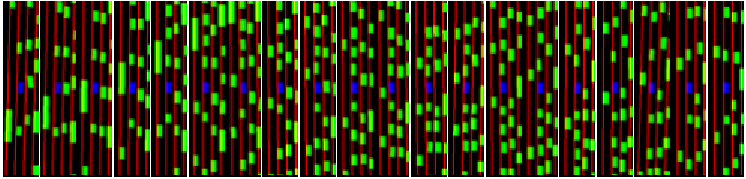
\includegraphics[width=0.95\textwidth]{figures/driving/video_predictions/truth-crop.pdf}} \\
    \subfigure[Deterministic Model]{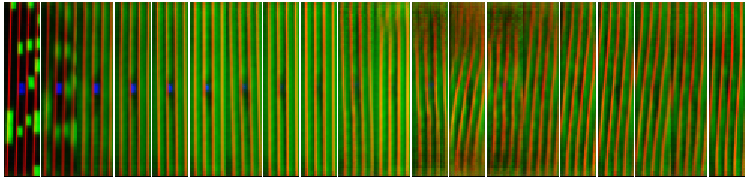
\includegraphics[width=0.95\textwidth]{figures/driving/video_predictions/det-crop.pdf}} \\
    \subfigure[Stochastic Model, sample 1]{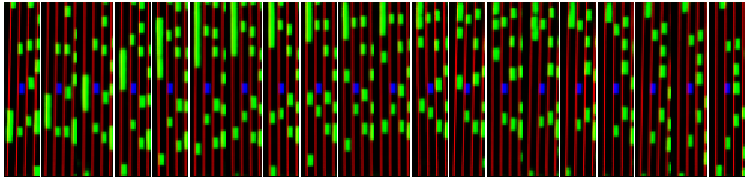
\includegraphics[width=0.95\textwidth]{figures/driving/video_predictions/pred1-crop.pdf}} \\
    \subfigure[Stochastic Model, sample 2]{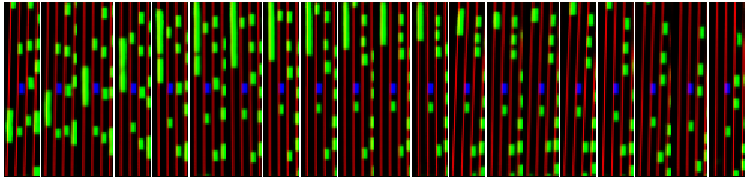
\includegraphics[width=0.95\textwidth]{figures/driving/video_predictions/pred2-crop.pdf}} \\
    \label{prediction-results}
    \caption{Video prediction results using a deterministic and stochastic model. Two different future predictions are generated by the stochastic model by sampling two different sequences of latent variables. The deterministic model averages over possible futures, producing blurred predictions.}
\end{figure*}









    \subsection{Planning Results}

    We now give results for planning, with performance measured in terms of episode length. An episode terminates when a car collides with another car, drives off the road or reaches the end of the road segment. Lower episode lengths indicate more collisions. All cars are initialized at the beginning of the road segment with the initial speed they were driving at in the dataset, and then controlled by the policy being measured. Since there is considerable variation in episode length, we report both the median and the mean. Table \ref{main-table} compares performance for the different methods described in Section \ref{planning-methods}.

    Both the SMPC and SVG methods require optimizing a differentiable cost function. We used the following:

    \begin{equation}
      C = C_{proximity} + 0.1 \cdot C_{lane} + \lambda_U \cdot C_U
    \end{equation}

    where $C_{proximity}$ and $C_{lane}$ are the proximity and lane costs described in Section \ref{i80-dataset-prep}, and $C_U$ is the differentiable epistemic uncertainty cost described in Section 5.5. We compare results with $\lambda_U = 0$ and $\lambda_U > 0$ to show its effect.

    \textbf{Training Details:} All policy networks have the same architecture: a 3-layer ConvNet with feature maps of size 64-128-256, followed by 3 fully-connected layers with 256 hidden units each, with the last layer outputting the parameters of a 2D Gaussian distribution over actions. All policy networks are trained with Adam with learning rate 0.0001. The SMBIL and SVG policies are trained by backpropagation through the unrolled forward model using the reparamaterization trick \citep{VAE}. The single-step imitation learner is trained to directly minimize the negative log-likelihood of the ground truth action in the dataset under the parameters output by the policy network. Both SMPC and SVG models unroll the forward model for 20 steps, and we report results for different unrolling lengths for SMBIL policies.
    The gradient descent procedure for the SMPC planner performs 5 gradient steps using Adam with learning rate 0.1. Actions are initialized to zero for the first time step, after which we used the rotating action buffer described in Section \ref{MPC}. We sampled 10 sequences of latent variables. We also provide a comparison without the buffer in the next section.

  \begin{table}[t]
    \centering
  \begin{tabular}{|lll|}
    \hline
    Method & Ep. Length & Planning Time \\
    \hhline{|===|}
    No action & 13.0 & 0 \\
    \hline
    1-step IL & 6.78 & 1 \\
    SMBIL (1 step) & 5.96 & 1 \\
    SMBIL (3 step) & 7.18 & 1 \\
    SMBIL (5 step) & 10.4 & 1 \\
    SMBIL (10 step) & 8.87 & 1 \\
    SMBIL (20 step) & 8.83 & 1 \\
    \hline
    SMPC-TEN (20 steps), $\lambda_U=0$ & 9.6 & 200 \\
    SMPC-TEN (20 steps), $\lambda_U=0.01$ & \textbf{28.6} & 2000 \\
    \hline
    SVG-TEN (20 steps), $\lambda_U=0$ & 2.61 & 1 \\
    SVG-TEN (20 steps), $\lambda_U=0.01$ & \textbf{29.6} & 1 \\
    \hline
  \end{tabular}
  \caption{Planning performance on NGSIM dataset, measured in mean episode length. An episode ends when the controlled car collides with another car, drives off the road or reaches the end of the road segment.}
  \label{main-table}
  \end{table}


  The 1-step imitation learner performs similarly to the SMBIL policy with a single step prediction.
  Training SMBIL policies with longer rollouts improves performance up to a point, but still does not beat the simple baseline of performing no action.
  Both SMPC and SVG without the uncertainty cost also give poor performance.
  However, adding the uncertainty cost improves performance dramatically, outperforming all other methods by a wide margin.
  Planning with the SMPC was very computationally demanding and the results we report are only over the first 100 trajectories (out of 278) in the test set, which still took over 36 hours wallclock time.
  In contrast, SVG with the uncertainty penalty is both fast and effective.
  Videos of the learned policies driving in the environment can be found at \url{https://youtu.be/ApjHjhyAMw0}.
  The policy learns effective behaviors such as braking, accelerating and turning to avoid other cars.

\begin{figure*}[t!]
    \centering
    \subfigure[$\lambda_U=0.01$]{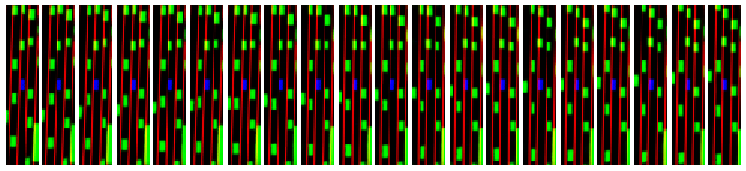
\includegraphics[width=0.95\textwidth]{figures/driving/svg_reg_prediction-crop.pdf}} \\
    \subfigure[$\lambda_U=0$]{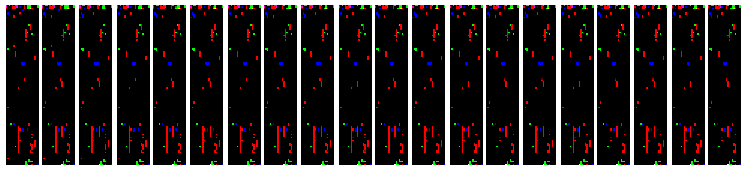
\includegraphics[width=0.95\textwidth]{figures/driving/svg_no_reg_prediction-crop.pdf}} \\

    \subfigure{

  \begin{tabular}{|llll|}
    \hline
    Method & Ep. Length & Predicted cost & $C_U$ \\
    \hhline{|====|}
    SVG-TEN, $\lambda_U=0.01$ & 29.6 & 0.0830 & 1.451 \\
    SVG-TEN, $\lambda_U=0$ & 2.6 & 0.0005 & 8717 \\
    \hline
  \end{tabular}
}
%  Executing these actions in the environment gives very poor performance, as shown in Table \ref{main-table}.
    \caption{Predictions made by the same forward model for an action sequence produced by a policy trained \textit{with} (top) and \textit{without} (bottom) the epistemic uncertainty cost. Without the uncertainty cost, the policy network learns to output pathological action sequences which produce invalid predictions which nevertheless have low cost.}
    \label{svg-pred}
\end{figure*}

  To illustrate the effect of the epistemic uncertainty cost, we plot predictions made by the forward model for an action sequence produced by SVG policy networks trained with and without the epistemic uncertainty cost, shown in Figure \ref{svg-pred}.
  The policy network trained with the uncertainty cost produces actions which, when plugged into the forward model, yield predictions which remain on the data manifold.
  The policy network trained without the uncertainty cost, however, produces actions which produce predictions not resembling any of the training examples.
  Notice however that these predictions yield low proximity cost, since the green channel representing cars is almost zero.
  Also included in Figure \ref{svg-pred} are the average predicted proximity cost by the forward model for both policies, as well as average epistemic uncertainty cost $C_U$.
  The model trained without the uncertainty penalty produces actions for which the forward model predicts very low cost, but its uncertainty about its predictions is very high.
  The model trained with the penalty produces actions for which the forward model predicts higher cost, but with much less uncertainty.
  Including the uncertainty cost forces the policy network to produce actions which still produce reasonable predictions under the forward model, and give much better results when executed in the environment.



  We additionally performed several ablation experiments to understand the effects of different modeling choices, shown in table \ref{ablation}.
  Using the action buffer has a non-negligible effect on the SMPC planning, as we see a performance drop when starting from newly initialized actions every time planning is required rather than initializing with a previously optimized action sequence.
  It is possible that with larger numbers of gradient steps this difference in performance would decrease, but the current setup is already very expensive.
  We also compared our TEN model to a VAE model with the same architecture and hyperparameters, except for the $\beta$ hyperparameter representing the weight of the KL term in the loss, which we set to $10^{-6}$ (we optimized over the range $\{ 1, 10^{-1},..., 10^{-6} \}$ and found that values higher than $10^{-5}$ produced blurry predictions similar to the deterministic model.
  Performance is very similar for both models.

  Finally, we compare SVG performance with and without masking the $z$ variables during training.
  Not including the masking causes a performance drop due to the forward model becoming less sensitive to the actions.




  \begin{table}[t]
    \centering
  \begin{tabular}{|lll|}
    \hline
    Method & Ep. Length & Planning Time \\
    \hhline{|===|}
    SMPC-TEN & 28.6  & 2000 \\
    SMPC-VAE & 28.4 & 2000 \\
    SMPC-TEN, no action buffer & 22.6 & 2000 \\
    \hline
    SVG-TEN & 29.6 & 1 \\
    SVG-TEN, no $z$ masking & 27.5 & 1 \\
    \hline
  \end{tabular}
  \caption{Ablation experiments. SMPC-VAE represents the SMPC method using a VAE instead of a TEN as a forward model.}
  \label{ablation}
  \end{table}


  \section{Conclusion}

  In this chapter we have presented an end-to-end approach for learning driving policies from observational data, which includes preparing a dataset of real-world driving trajectories, adapting it to become a planning environment, training a stochastic forward model, and using it for planning together with a new uncertainty regularizer which solves the domain mismatch problem.
  There are several directions for future work.
  First, our current approach does not capture dependencies which are longer than 20 time steps into the future, which corresponds to 2 seconds.
  We tried two different approaches to capture longer-term dependencies: learning a value function using temporal differences (which in theory can capture arbitrary length dependencies) and unrolling for more time steps, but these did not yield any improvements and sometimes hurt performance. This requires more investigation.
%  Second, we observed that the latent variables still encoded action information, although adding the dropout on the latent variables reduced this problem.
%  Finding a more principled method would be an interesting direction for future work.
  Second, it would be interesting to optimize actions or policies to produce more complex and useful behaviors, such as changing to a specified lane while avoiding other cars.
  In the current setup, the policies are optimized only to avoid collisions and stay within lanes when possible, whereas in a real-world scenario we would want a policy which can safely navigate among traffic to different locations.


\section{General formatting instructions}
\label{gen_inst}

The text must be confined within a rectangle 5.5~inches (33~picas) wide and
9~inches (54~picas) long. The left margin is 1.5~inch (9~picas).
Use 10~point type with a vertical spacing of 11~points. Times New Roman is the
preferred typeface throughout. Paragraphs are separated by 1/2~line space,
with no indentation.

Paper title is 17~point, in small caps and left-aligned.
All pages should start at 1~inch (6~picas) from the top of the page.

Authors' names are
set in boldface, and each name is placed above its corresponding
address. The lead author's name is to be listed first, and
the co-authors' names are set to follow. Authors sharing the
same address can be on the same line.

Please pay special attention to the instructions in section \ref{others}
regarding figures, tables, acknowledgments, and references.

\section{Headings: first level}
\label{headings}

First level headings are in small caps,
flush left and in point size 12. One line space before the first level
heading and 1/2~line space after the first level heading.

\subsection{Headings: second level}

Second level headings are in small caps,
flush left and in point size 10. One line space before the second level
heading and 1/2~line space after the second level heading.

\subsubsection{Headings: third level}

Third level headings are in small caps,
flush left and in point size 10. One line space before the third level
heading and 1/2~line space after the third level heading.

\section{Citations, figures, tables, references}
\label{others}

These instructions apply to everyone, regardless of the formatter being used.

\subsection{Citations within the text}

Citations within the text should be based on the \texttt{natbib} package
and include the authors' last names and year (with the ``et~al.'' construct
for more than two authors). When the authors or the publication are
included in the sentence, the citation should not be in parenthesis (as
in ``See \citet{Hinton06} for more information.''). Otherwise, the citation
should be in parenthesis (as in ``Deep learning shows promise to make progress towards AI~\citep{Bengio+chapter2007}.'').

The corresponding references are to be listed in alphabetical order of
authors, in the \textsc{References} section. As to the format of the
references themselves, any style is acceptable as long as it is used
consistently.

\subsection{Footnotes}

Indicate footnotes with a number\footnote{Sample of the first footnote} in the
text. Place the footnotes at the bottom of the page on which they appear.
Precede the footnote with a horizontal rule of 2~inches
(12~picas).\footnote{Sample of the second footnote}

\subsection{Figures}

All artwork must be neat, clean, and legible. Lines should be dark
enough for purposes of reproduction; art work should not be
hand-drawn. The figure number and caption always appear after the
figure. Place one line space before the figure caption, and one line
space after the figure. The figure caption is lower case (except for
first word and proper nouns); figures are numbered consecutively.

Make sure the figure caption does not get separated from the figure.
Leave sufficient space to avoid splitting the figure and figure caption.

You may use color figures.
However, it is best for the
figure captions and the paper body to make sense if the paper is printed
either in black/white or in color.
\begin{figure}[h]
\begin{center}
%\framebox[4.0in]{$\;$}
\fbox{\rule[-.5cm]{0cm}{4cm} \rule[-.5cm]{4cm}{0cm}}
\end{center}
\caption{Sample figure caption.}
\end{figure}

\subsection{Tables}

All tables must be centered, neat, clean and legible. Do not use hand-drawn
tables. The table number and title always appear before the table. See
Table~\ref{sample-table}.

Place one line space before the table title, one line space after the table
title, and one line space after the table. The table title must be lower case
(except for first word and proper nouns); tables are numbered consecutively.

\begin{table}[t]
\caption{Sample table title}
\label{sample-table}
\begin{center}
\begin{tabular}{ll}
\multicolumn{1}{c}{\bf PART}  &\multicolumn{1}{c}{\bf DESCRIPTION}
\\ \hline \\
Dendrite         &Input terminal \\
Axon             &Output terminal \\
Soma             &Cell body (contains cell nucleus) \\
\end{tabular}
\end{center}
\end{table}

\section{Default Notation}

In an attempt to encourage standardized notation, we have included the
notation file from the textbook, \textit{Deep Learning}
\cite{goodfellow2016deep} available at
\url{https://github.com/goodfeli/dlbook_notation/}.  Use of this style
is not required and can be disabled by commenting out
\texttt{math\_commands.tex}.


\centerline{\bf Numbers and Arrays}
\bgroup
\def\arraystretch{1.5}
\begin{tabular}{p{1in}p{3.25in}}
$\displaystyle a$ & A scalar (integer or real)\\
$\displaystyle \va$ & A vector\\
$\displaystyle \mA$ & A matrix\\
$\displaystyle \tA$ & A tensor\\
$\displaystyle \mI_n$ & Identity matrix with $n$ rows and $n$ columns\\
$\displaystyle \mI$ & Identity matrix with dimensionality implied by context\\
$\displaystyle \ve^{(i)}$ & Standard basis vector $[0,\dots,0,1,0,\dots,0]$ with a 1 at position $i$\\
$\displaystyle \text{diag}(\va)$ & A square, diagonal matrix with diagonal entries given by $\va$\\
$\displaystyle \ra$ & A scalar random variable\\
$\displaystyle \rva$ & A vector-valued random variable\\
$\displaystyle \rmA$ & A matrix-valued random variable\\
\end{tabular}
\egroup
\vspace{0.25cm}

\centerline{\bf Sets and Graphs}
\bgroup
\def\arraystretch{1.5}

\begin{tabular}{p{1.25in}p{3.25in}}
$\displaystyle \sA$ & A set\\
$\displaystyle \R$ & The set of real numbers \\
$\displaystyle \{0, 1\}$ & The set containing 0 and 1 \\
$\displaystyle \{0, 1, \dots, n \}$ & The set of all integers between $0$ and $n$\\
$\displaystyle [a, b]$ & The real interval including $a$ and $b$\\
$\displaystyle (a, b]$ & The real interval excluding $a$ but including $b$\\
$\displaystyle \sA \backslash \sB$ & Set subtraction, i.e., the set containing the elements of $\sA$ that are not in $\sB$\\
$\displaystyle \gG$ & A graph\\
$\displaystyle \parents_\gG(\ervx_i)$ & The parents of $\ervx_i$ in $\gG$
\end{tabular}
\vspace{0.25cm}


\centerline{\bf Indexing}
\bgroup
\def\arraystretch{1.5}

\begin{tabular}{p{1.25in}p{3.25in}}
$\displaystyle \eva_i$ & Element $i$ of vector $\va$, with indexing starting at 1 \\
$\displaystyle \eva_{-i}$ & All elements of vector $\va$ except for element $i$ \\
$\displaystyle \emA_{i,j}$ & Element $i, j$ of matrix $\mA$ \\
$\displaystyle \mA_{i, :}$ & Row $i$ of matrix $\mA$ \\
$\displaystyle \mA_{:, i}$ & Column $i$ of matrix $\mA$ \\
$\displaystyle \etA_{i, j, k}$ & Element $(i, j, k)$ of a 3-D tensor $\tA$\\
$\displaystyle \tA_{:, :, i}$ & 2-D slice of a 3-D tensor\\
$\displaystyle \erva_i$ & Element $i$ of the random vector $\rva$ \\
\end{tabular}
\egroup
\vspace{0.25cm}


\centerline{\bf Calculus}
\bgroup
\def\arraystretch{1.5}
\begin{tabular}{p{1.25in}p{3.25in}}
% NOTE: the [2ex] on the next line adds extra height to that row of the table.
% Without that command, the fraction on the first line is too tall and collides
% with the fraction on the second line.
$\displaystyle\frac{d y} {d x}$ & Derivative of $y$ with respect to $x$\\ [2ex]
$\displaystyle \frac{\partial y} {\partial x} $ & Partial derivative of $y$ with respect to $x$ \\
$\displaystyle \nabla_\vx y $ & Gradient of $y$ with respect to $\vx$ \\
$\displaystyle \nabla_\mX y $ & Matrix derivatives of $y$ with respect to $\mX$ \\
$\displaystyle \nabla_\tX y $ & Tensor containing derivatives of $y$ with respect to $\tX$ \\
$\displaystyle \frac{\partial f}{\partial \vx} $ & Jacobian matrix $\mJ \in \R^{m\times n}$ of $f: \R^n \rightarrow \R^m$\\
$\displaystyle \nabla_\vx^2 f(\vx)\text{ or }\mH( f)(\vx)$ & The Hessian matrix of $f$ at input point $\vx$\\
$\displaystyle \int f(\vx) d\vx $ & Definite integral over the entire domain of $\vx$ \\
$\displaystyle \int_\sS f(\vx) d\vx$ & Definite integral with respect to $\vx$ over the set $\sS$ \\
\end{tabular}
\egroup
\vspace{0.25cm}

\centerline{\bf Probability and Information Theory}
\bgroup
\def\arraystretch{1.5}
\begin{tabular}{p{1.25in}p{3.25in}}
$\displaystyle P(\ra)$ & A probability distribution over a discrete variable\\
$\displaystyle p(\ra)$ & A probability distribution over a continuous variable, or over
a variable whose type has not been specified\\
$\displaystyle \ra \sim P$ & Random variable $\ra$ has distribution $P$\\% so thing on left of \sim should always be a random variable, with name beginning with \r
$\displaystyle  \E_{\rx\sim P} [ f(x) ]\text{ or } \E f(x)$ & Expectation of $f(x)$ with respect to $P(\rx)$ \\
$\displaystyle \Var(f(x)) $ &  Variance of $f(x)$ under $P(\rx)$ \\
$\displaystyle \Cov(f(x),g(x)) $ & Covariance of $f(x)$ and $g(x)$ under $P(\rx)$\\
$\displaystyle H(\rx) $ & Shannon entropy of the random variable $\rx$\\
$\displaystyle \KL ( P \Vert Q ) $ & Kullback-Leibler divergence of P and Q \\
$\displaystyle \mathcal{N} ( \vx ; \vmu , \mSigma)$ & Gaussian distribution %
over $\vx$ with mean $\vmu$ and covariance $\mSigma$ \\
\end{tabular}
\egroup
\vspace{0.25cm}

\centerline{\bf Functions}
\bgroup
\def\arraystretch{1.5}
\begin{tabular}{p{1.25in}p{3.25in}}
$\displaystyle f: \sA \rightarrow \sB$ & The function $f$ with domain $\sA$ and range $\sB$\\
$\displaystyle f \circ g $ & Composition of the functions $f$ and $g$ \\
  $\displaystyle f(\vx ; \vtheta) $ & A function of $\vx$ parametrized by $\vtheta$.
  (Sometimes we write $f(\vx)$ and omit the argument $\vtheta$ to lighten notation) \\
$\displaystyle \log x$ & Natural logarithm of $x$ \\
$\displaystyle \sigma(x)$ & Logistic sigmoid, $\displaystyle \frac{1} {1 + \exp(-x)}$ \\
$\displaystyle \zeta(x)$ & Softplus, $\log(1 + \exp(x))$ \\
$\displaystyle || \vx ||_p $ & $\normlp$ norm of $\vx$ \\
$\displaystyle || \vx || $ & $\normltwo$ norm of $\vx$ \\
$\displaystyle x^+$ & Positive part of $x$, i.e., $\max(0,x)$\\
$\displaystyle \1_\mathrm{condition}$ & is 1 if the condition is true, 0 otherwise\\
\end{tabular}
\egroup
\vspace{0.25cm}



\section{Final instructions}
Do not change any aspects of the formatting parameters in the style files.
In particular, do not modify the width or length of the rectangle the text
should fit into, and do not change font sizes (except perhaps in the
\textsc{References} section; see below). Please note that pages should be
numbered.

\section{Preparing PostScript or PDF files}

Please prepare PostScript or PDF files with paper size ``US Letter'', and
not, for example, ``A4''. The -t
letter option on dvips will produce US Letter files.

Consider directly generating PDF files using \verb+pdflatex+
(especially if you are a MiKTeX user).
PDF figures must be substituted for EPS figures, however.

Otherwise, please generate your PostScript and PDF files with the following commands:
\begin{verbatim}
dvips mypaper.dvi -t letter -Ppdf -G0 -o mypaper.ps
ps2pdf mypaper.ps mypaper.pdf
\end{verbatim}

\subsection{Margins in LaTeX}

Most of the margin problems come from figures positioned by hand using
\verb+\special+ or other commands. We suggest using the command
\verb+\includegraphics+
from the graphicx package. Always specify the figure width as a multiple of
the line width as in the example below using .eps graphics
\begin{verbatim}
   \usepackage[dvips]{graphicx} ...
   \includegraphics[width=0.8\linewidth]{myfile.eps}
\end{verbatim}
or % Apr 2009 addition
\begin{verbatim}
   \usepackage[pdftex]{graphicx} ...
   \includegraphics[width=0.8\linewidth]{myfile.pdf}
\end{verbatim}
for .pdf graphics.
See section~4.4 in the graphics bundle documentation (\url{http://www.ctan.org/tex-archive/macros/latex/required/graphics/grfguide.ps})

A number of width problems arise when LaTeX cannot properly hyphenate a
line. Please give LaTeX hyphenation hints using the \verb+\-+ command.


\subsubsection*{Acknowledgments}

Use unnumbered third level headings for the acknowledgments. All
acknowledgments, including those to funding agencies, go at the end of the paper.

\bibliography{iclr2019_conference}
\bibliographystyle{iclr2019_conference}

\end{document}
